% ****** Start of file aipsamp.tex ******
%
%   This file is part of the AIP files in the AIP distribution for REVTeX 4.
%   Version 4.1 of REVTeX, October 2009
%
%   Copyright (c) 2009 American Institute of Physics.
%
%   See the AIP README file for restrictions and more information.
%
% TeX'ing this file requires that you have AMS-LaTeX 2.0 installed
% as well as the rest of the prerequisites for REVTeX 4.1
% 
% It also requires running BibTeX. The commands are as follows:
%
%  1)  latex  aipsamp
%  2)  bibtex aipsamp
%  3)  latex  aipsamp
%  4)  latex  aipsamp
%
% Use this file as a source of example code for your aip document.
% Use the file aiptemplate.tex as a template for your document.
\documentclass[%
 aip,
% jmp,
% bmf,
% sd,
% rsi,
 amsmath,amssymb,
%preprint,%
 reprint,%
%author-year,%
%author-numerical,%
% Conference Proceedings
]{revtex4-1}

\usepackage{graphicx}% Include figure files
\usepackage{dcolumn}% Align table columns on decimal point
\usepackage{bm}% bold math
%\usepackage[mathlines]{lineno}% Enable numbering of text and display math
%\linenumbers\relax % Commence numbering lines

\usepackage[utf8]{inputenc}
\usepackage[T1]{fontenc}
\usepackage{mathptmx}
\usepackage{etoolbox}
\usepackage{booktabs}
\usepackage{multirow}
\usepackage{gensymb}
\usepackage{siunitx}
\usepackage{bm}
\DeclareSIUnit\gauss{G}
\usepackage[hidelinks]{hyperref}
\hypersetup{
    colorlinks=true,
    linkcolor=blue,
    filecolor=magenta,      
    urlcolor=cyan,
    pdftitle={Overleaf Example},
    pdfpagemode=FullScreen,
    }

%% Apr 2021: AIP requests that the corresponding 
%% email to be moved after the affiliations
\makeatletter
\def\@email#1#2{%
 \endgroup
 \patchcmd{\titleblock@produce}
  {\frontmatter@RRAPformat}
  {\frontmatter@RRAPformat{\produce@RRAP{*#1\href{mailto:#2}{#2}}}\frontmatter@RRAPformat}
  {}{}
}%
\makeatother
\begin{document}

\preprint{AIP/123-QED}

\title[Hall effect and magnetoresistance in semiconductors]{Hall effect and magnetoresistance in semiconductors}
% Force line breaks with \\
\author{Maitrey Sharma}
 \affiliation{School of Physical Sciences, National Institute of Science Education and Research, HBNI, Jatni-752050, India.}%Lines break automatically or can be forced with \\
 \email{maitrey.sharma@niser.ac.in}

\date{\today}% It is always \today, today,
             %  but any date may be explicitly specified

\begin{abstract}
This experiment primarily deals with the study of the phenomena of Hall effect and magneto-resistance in semiconductors. First we explore the Drude model to lay down the foundation for the concepts and origin of Hall voltage and magneto-resistance and then using the well-known instrumentation like the four-probe, we establish various results. We determine the Hall coefficients of Bi, p-Ge and n-Ge and its relation to carrier density and carrier mobility, which are also determined for Bi. The unusual case of Bi is especially studied theoretically and experimentally. Then the magneto-resistance of Bi and n-Ge is determined and several plots are studied and results are drawn regarding them. 
\end{abstract}

\maketitle 


\begin{quotation}
\textit{There is nothing in the world except empty curved space. Matter, charge, electromagnetism, and other fields are only manifestations of the curvature of space.}
\newline
\hspace*{0pt}\hfill John Wheeler
\end{quotation}

\section{Introduction}
    When a current-carrying conductor is placed in a magnetic field perpendicular to the current direction, a voltage develops transverse to the current. This voltage was first observed in 1879 by Edwin Hall and this effect is called \textit{Hall Effect}.
    \par
    The Hall effect has since led to a deeper understanding of the details of the conduction process. It can yield the density of the charge carriers as well as their sign. In simple metals, the density of carriers is an integer multiple of the density of atoms; this indicates that each atom donates a fixed number of electrons to the conduction process. In more complex metals such as bismuth, the conduction based has a small overlap with the valence band, which then contributors a very small number of electrons to the conduction band loading to very low carrier density.
    \par
    The first part of the experiment concerns with study of the Hall effect in Bismuth, n-type Germanium and p-type Germanium. The second part deals with the phenomena of magnetoresistance, which follows from the concept of carrier mobility.
    \par
    It is noticed that the resistance of a sample changes when the magnetic field is turned on. The \textit{magneto-resistance} is the property of a material to change the value of its electrical resistance when an external magnetic field is applied to it. The effect was first discovered by William Thomson (more commonly known as Lord Kelvin) in 1856.
    \par
    Magneto-resistance, is due to the fact that the drift velocity of all the carriers is not same, and the mechanism of which will be understood in depth using the \textbf{Drude model} later in the theory section.
    \begin{figure}
        \centering
        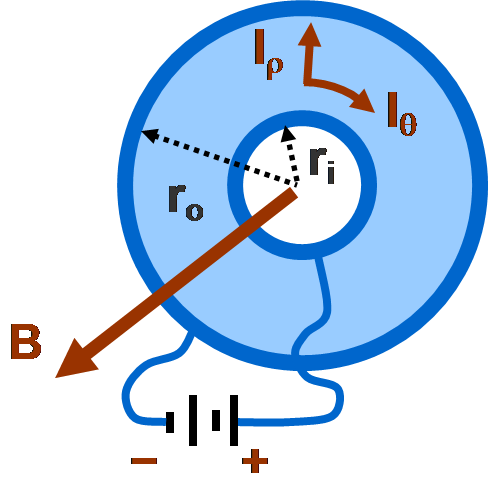
\includegraphics[scale = 0.35]{Figures/Corbino_disc.png}
        \caption{Corbino disc. With the magnetic field turned off, a radial current flows in the conducting annulus due to the battery connected between the (infinite) conductivity rims. When a magnetic field along the axis is turned on (B points directly out of the screen), the Lorentz force drives a circular component of current, and the resistance between the inner and outer rims goes up. This increase in resistance due to the magnetic field is called magnetoresistance.}
        \label{fig:my_label}
    \end{figure}
\section{Aim}
    \begin{itemize}
        \item To study the Hall effect and determine the Hall coefficient at ambient temperature for various samples of semiconductors.
        \item To study the magneto-resistance of various samples of semiconductors.
    \end{itemize}
\section{Apparatus}
    The apparatus used throughout the experiment is:
    \begin{enumerate}
        \item Hall Probe (Bismuth),
        \item Four probe arrangement,
        \item Samples of the semiconductors used in the experiment (Bi, n-Ge, p-Ge)
        \item Constant Current Source, CCS-01,
        \item Digital Microvoltmeter, DMV-001,
        \item Electromagnet, Model EMU-75,
        \item Constant Current Power Supply, DPS-175, 
        \item Digital Gaussmeter, DGM-102, 
        \item Hall Probe Stand
    \end{enumerate}


\section{Experimental set-up}
    \subsection{Hall Probe (Bismuth)}
    Bismuth strip with four spring type pressure contacts is mounted on a sunmica decorated bakelite strip Four leads are provided for connections with measuring devices.
    \subsection{Constant Current Source, Model : CCS-01}
    It is an IC regulated current generator to provide a constant current to the outer probes irrespective of the changing resistance of the sample due to change in temperatures. The basic scheme is to use the feedback principle to limit the load current of the supply to preset maximum value. Variations in the current are achieved by a potentiometer included for that purpose. The supply is a highly regulated and practically ripples free $DC$ source. The constant current source is suitable for the resistivity measurement of thin films of metals/ alloys and semiconductors like germanium.
    \subsection{DC Microvoltmeter, Model DMV-001}
    Digital Microvoltmeter, DMV-001 is a very versatile multipurpose instrument
    for the measurement of low $DC$ voltage. It has 5 decade ranges from $\SI{1}{\milli \volt}$ to $\SI{10}{\volt}$ with
    100\% over-ranging. This instrument uses a very well designed chopper stabilized IC amplifier.
    This amplifier offers exceptionally low offset voltage and input bias parameters, combined with excellent speed characteristics.
    \subsection{Electromagnet, EMU-75}
    The following are the specifications of EMU-75 unit:
    \begin{itemize}
        \item \textit{Field intensity}: 11,000 $\pm$ 5\% $\si{\gauss}$ in an air-gap of $\SI{10}{\milli \metre}$. Air-gap is continuously variable upto $\SI{100}{\milli \metre}$ with two way knobbed wheel screw adjusting system.
        \item \textit{Pole pieces}: $\SI{75}{\milli \metre}$ diameter. Normally flat faced pole pieces are supplied with the magnet.
        \item \textit{Energising coils}: Two. Each coil is wound on non-magnetic formers and has a resistance of 12 ohms approx.
        \item \textit{Yoke material}: Mild steel
        \item \textit{Power requirement}: 0 - 100 $\si{\volt}$ @ $\SI{3.5}{\ampere}$ if connected in series; 0 - 50 $\si{\volt}$ @ $\SI{7.0}{\ampere}$ if connected in parallel.
    \end{itemize}
    \subsection{Constant Current Power Supply, DPS-175}
    The present constant current power supply was designed to be used with the
    electromagnet, Model EMU-75. The current requirement of 3.5 amp/coil, i.e. a total of 7
    Amp was met by connecting six closely matched constant current sources in parallel. In
    this arrangement the first unit works as the 'master' with current adjustment control. All
    others are 'slave' units, generating exactly the same current as the master.
    \subsection{Four Probes Arrangement}
    It has four individually spring loaded probes. The probes are collinear and
    equally spaced. The probes are mounted in a teflon bush, which ensure a good
    electrical insulation between the probes. A teflon spacer near the tips is also provided
    to keep the probes at equal distance. The probe arrangement is mounted in a suitable
    stand, which also holds the sample plate and RTD sensor. This stand also serves as
    the lid of PID Controlled Oven. Proper leads are provided for current, Voltage and
    Temp. measurement with their universal connectors. For current measurement there is
    three pin connector which can be connected to the CCS-01/ LCS-02 as per
    requirement of sample. For voltage measurement BNC connector is used connected to
    DMV-001 unit. For temperature measurement, a two pin connector is provided for
    connection with PID- Controlled oven unit PID-200 at connector marked as
    Temperature Sensor. Three levelling screws are provided in Four Probe arrangement by which we can adjust the
    level of plateform to make it horizontal. A probe holding screw is provided at the collar of the
    arrangement. Initially it should be in loose position, to allow free movement of Probe Pipe.
    After placing the sample the Probe Pipe should be lowered so that all four pins touches the
    sample. The pipe is further pressed very lightly so that the assured firm contact is made of all Four
    Pins with the sample. The probe holding screw is tightened at this position making the arrangement ready to use.
    \subsection{Digital Gaussmeter, Model DGM-102}
    The Gaussmeter operates on the principle of Hall Effect in semiconductors. A
    semiconductor material carrying current develops an electro-motive force, when placed
    in a magnetic field, in a direction perpendicular to the direction of both electric current
    and magnetic field. The magnitude of this e.m.f. is proportional to the field intensity if
    the current is kept constant, this e.m.f. is called the Hall Voltage.
    \begin{figure*}
        \centering
        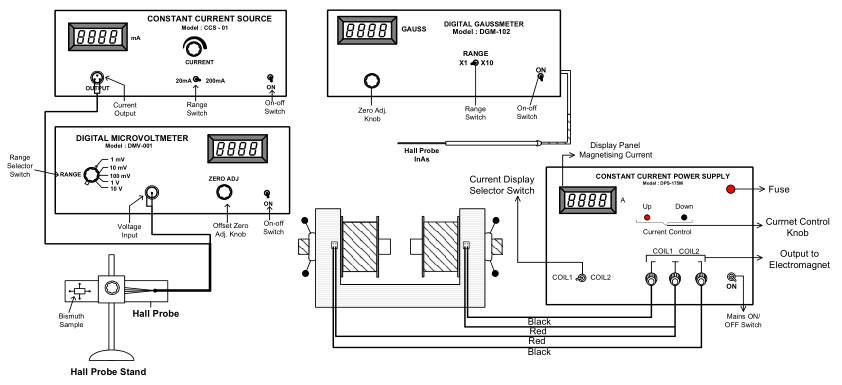
\includegraphics{Figures/panel-hall.png}
        \caption{Panel diagram for Hall effect experiment}
        \label{fig:my_label}
    \end{figure*}
    \begin{figure*}
        \centering
        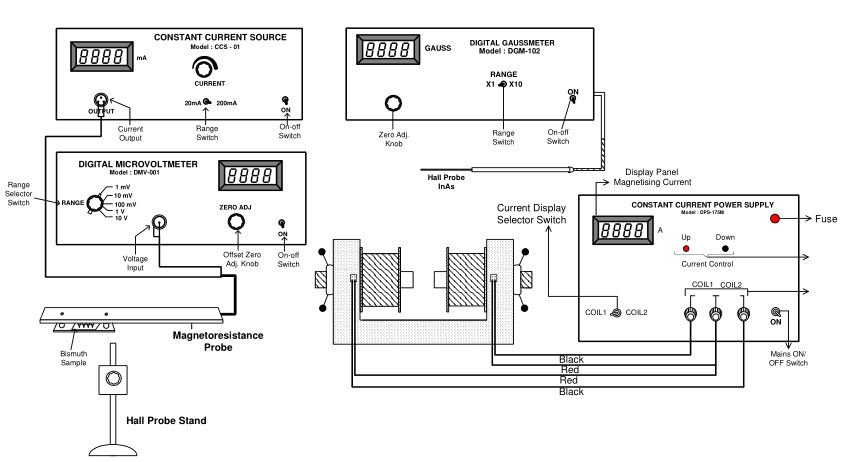
\includegraphics{Figures/panel-magneto.png}
        \caption{Panel diagram for magneto-resistance experiment}
        \label{fig:my_label}
    \end{figure*}
    \begin{figure}
        \centering
        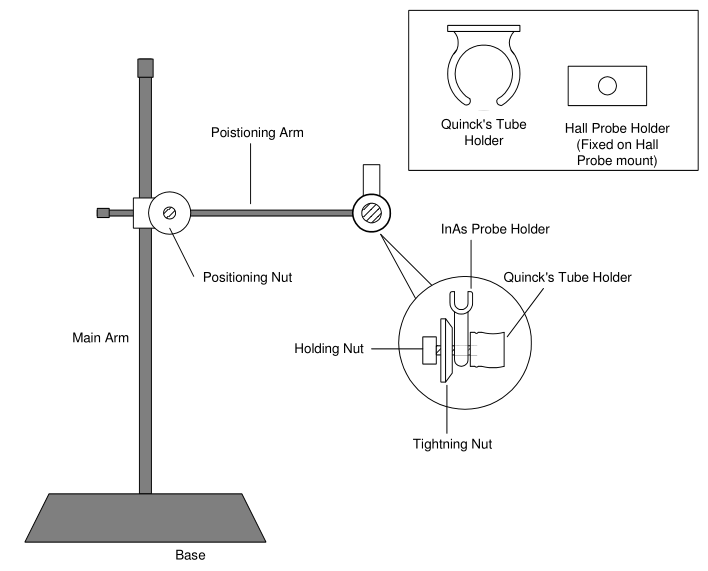
\includegraphics[scale = 0.5]{Figures/stand.png}
        \caption{Multi-purpose stand used in the experiments}
        \label{fig:my_label}
    \end{figure}
    \begin{figure}
        \centering
        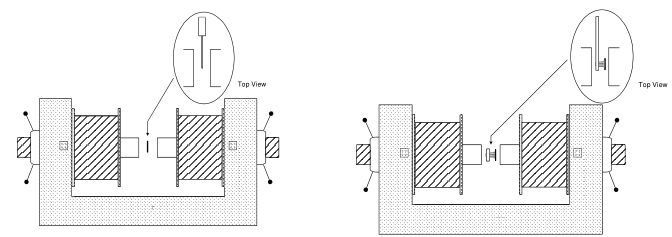
\includegraphics[scale = 0.5]{Figures/placing.png}
        \caption{The placing of Gaussmeter Hall probe in electromagnet (left) and of magneto-resistance sample in electromagnet (right)}
        \label{fig:my_label}
    \end{figure}
    \begin{figure}
        \centering
        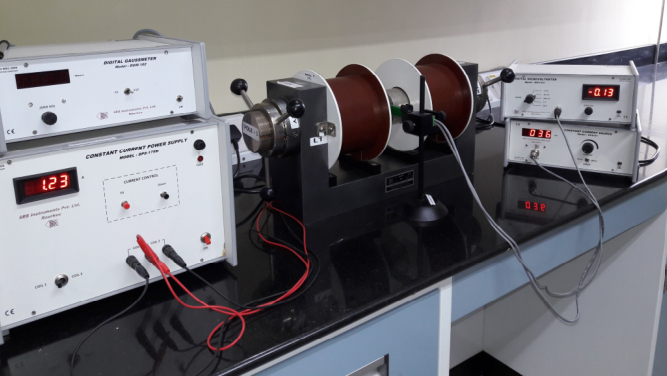
\includegraphics[scale = 0.5]{Figures/expt-setup.png}
        \caption{Complete experimental setup}
        \label{fig:my_label}
    \end{figure}

\section{Theory}
    \subsection{The Hall Effect}
    A static magnetic field has no effect on charges unless they are in motion. When the charges flow, a magnetic field directed perpendicular to the direction of
    flow produces a mutually perpendicular force on the charges. When this happens, electrons
    and holes will be separated by opposite forces. They will in turn produce an electric field ($\bm{E_h}$) which depends on the cross product of the magnetic intensity, $\bm{H}$, and the current density, $\bm{J}$. The situation is demonstrated in figure (\ref{fig:carrsep}).
    \begin{figure}
        \centering
        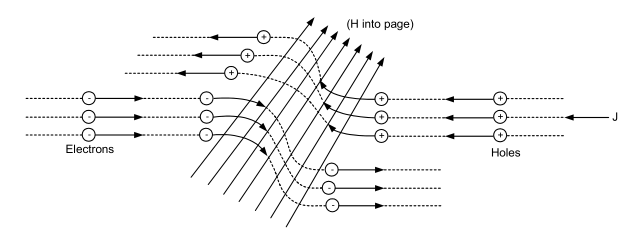
\includegraphics[scale = 0.62]{Figures/carr-sep-H.png}
        \caption{Carrier seperation due to a magnetic field}
        \label{fig:carrsep}
    \end{figure}
    \begin{figure}
        \centering
        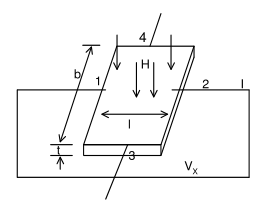
\includegraphics{Figures/hall-schematic.png}
        \caption{Schematic arrangement for the
measurement of Hall Effect of a crystal}
        \label{fig:my_label}
    \end{figure}
    \begin{equation}
        \bm{E_h} = R \bm{J} \times \bm{H}
    \end{equation}
    where $R$ is called the Hall coefficient.
    \par
    Now, let us consider a bar of a semiconductor, having dimensions, $x$, $y$ and $z$. Let $\bm{J}$ be
    directed along $X$ and $\bm{H}$ along $Z$, then
    $\bm{E_h}$ will be along $Y$, as in figure (\ref{fig:sampstudy}).
    \begin{figure}
        \centering
        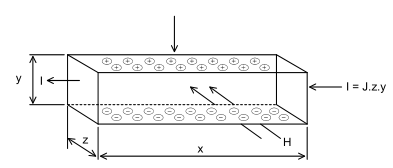
\includegraphics{Figures/study-hall.png}
        \caption{Sample for studying Hall Effect}
        \label{fig:sampstudy}
    \end{figure}
    Then,
    \begin{equation}
        R = \dfrac{V_h/y}{J H} = \dfrac{V_h \cdot z}{I H}
    \end{equation}
    where $V_h$ is the Hall voltage appearing between the two surfaces perpendicular to y and $I=Jyz$.
    \par
    In general, the Hall voltage is not a linear function of magnetic field applied, i.e. the
    Hall coefficient is not generally a constant, but a function of the applied magnetic field.
    Consequently, interpretation of the Hall Voltage is not usually a simple matter. However, it
    is easy to calculate this (Hall) voltage if it is assumed that all carriers have the same drift
    velocity. We will do this calculation for metals and degenerate (doped) semiconductors.
    \par
    The magnetic force on the carriers is $\bm{E_m} = e (\bm{v} \times \bm{H})$ and is compensated by the Hall
    field $\bm{F_h} = e \bm{E_h}$ where $\bm{v}$ is the drift velocity of the carrier. The current density is $\bm{J} = q n \bm{v}$. From here we get
    \begin{equation}
        R = \dfrac{E_h}{J H} = \dfrac{v \cdot H}{qnvH} = \dfrac{1}{nq}
    \end{equation}
    From this equation\footnote{assuming that all carriers have same velocity}, it is clear that the sign of Hall coefficient depend upon the sign of q. Also for a fixed magnetic field and input current, the Hall voltage is proportional to $1/n$ or its resistivity. The conductivity of the material is $\sigma = nq \mu$, where $\mu$ is the mobility of the charge carriers.
    \par
    Thus we see that the Hall coefficient, in conjunction with resistivity measurements, can provide information on carrier densities, mobilities, impurity concentration and other values.
    \subsection{Hall effect in Bismuth}
    Bi atoms have 5 valence electrons, two s electrons and 3 p electrons. The bulk
    crystal structure of Bi is a bit complicated but for us the only important thing is
    that there are two atoms per unit cell. This makes 10 electrons per unit cell. Since
    this is an even number, Bi could technically be a semiconductor but we need to
    keep in mind that having an even number of valence electrons per unit cell is only
    a necessary criterion for having a semiconductor. It is not sufficient. In the case
    of Bi, we have an electronic situation that is very close to being a semiconductor -
    but not quite.
    \par
    This is illustrate in figure \ref{fig:bihall}(a) which shows the band structure of Bi. The two
    lowest bands can be viewed as s-derived. The are well separated from the higher
    p-type bands and fully occupied by the 4 s electrons in the unit cell. this leaves
    6 p electrons which could exactly fill three more bands. A superficial look on the
    band structure appears to confirm this. When zooming in as schematically done
    in Figure \ref{fig:bihall}(b), however, we see that the upper “valence band” crosses the Fermi
    energy the T point of the Brillouin zone whereas the lowest “conduction band”
    drops below the Fermi energy at the L point. The valence band is thus almost
    completely filled apart from a very small concentration of holes and the conduction
    band is completely empty apart from a very small concentration of electrons. The
    total electron and hole concentration must the the same, of course, so that the Bi
    remains charge neutral. An impressive illustration of the small carrier concentration
    is shown in density of states shown Figure \ref{fig:bihall}(c). At first glance the density of states
    appears to go to zero near the Fermi energy such that a gap is formed. But this is
    so only superficially. The density of states does not actually go to zero. It is just
    very small.
    \begin{figure}
        \centering
        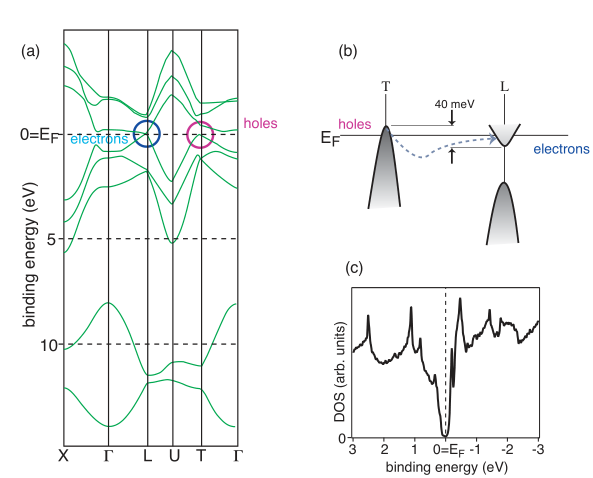
\includegraphics[scale = 0.65]{Figures/bi-hall.png}
        \caption{Electronic structure of Bismuth. (a) Bulk band dispersion in different directions of the Brillouin zone (b) Schematic band structure of the bands crossing the Fermi energy. (c) Density of states.}
        \label{fig:bihall}
    \end{figure}
    \subsection{Magneto-resistance in semiconductors}
    With the magnetic field on; the Hall voltage compensates exactly the Lorentz force for carriers with average velocity; slower carriers will be over compensated and faster ones undercompensated, resulting in trajectories that are not along the applied field.
    This results in an effective decrease of the mean free path and hence an increase in resistivity.
    Here the above referred symbols are defined as: $v =$ drift velocity; $E =$ applied electric field; $t
    =$ thickness of the crystal; $H =$ Magnetic field
    \subsection{Magneto-resistance in Bismuth}
    Bismuth is a semimetal. A semimetal is a material with a very small overlap between
    the bottom of the conduction band and the top of the valence band. Because of the slight overlap
    between the conduction and valence bands, semimetal has no band gap and a negligible density
    of states at the Fermi level. A metal, by contrast, has an appreciable density of states at the
    Fermi level because the conduction band is partially filled. Unlike metals, semimetals have
    both type of charge carriers viz. electrons and holes.
    \begin{figure}
        \centering
        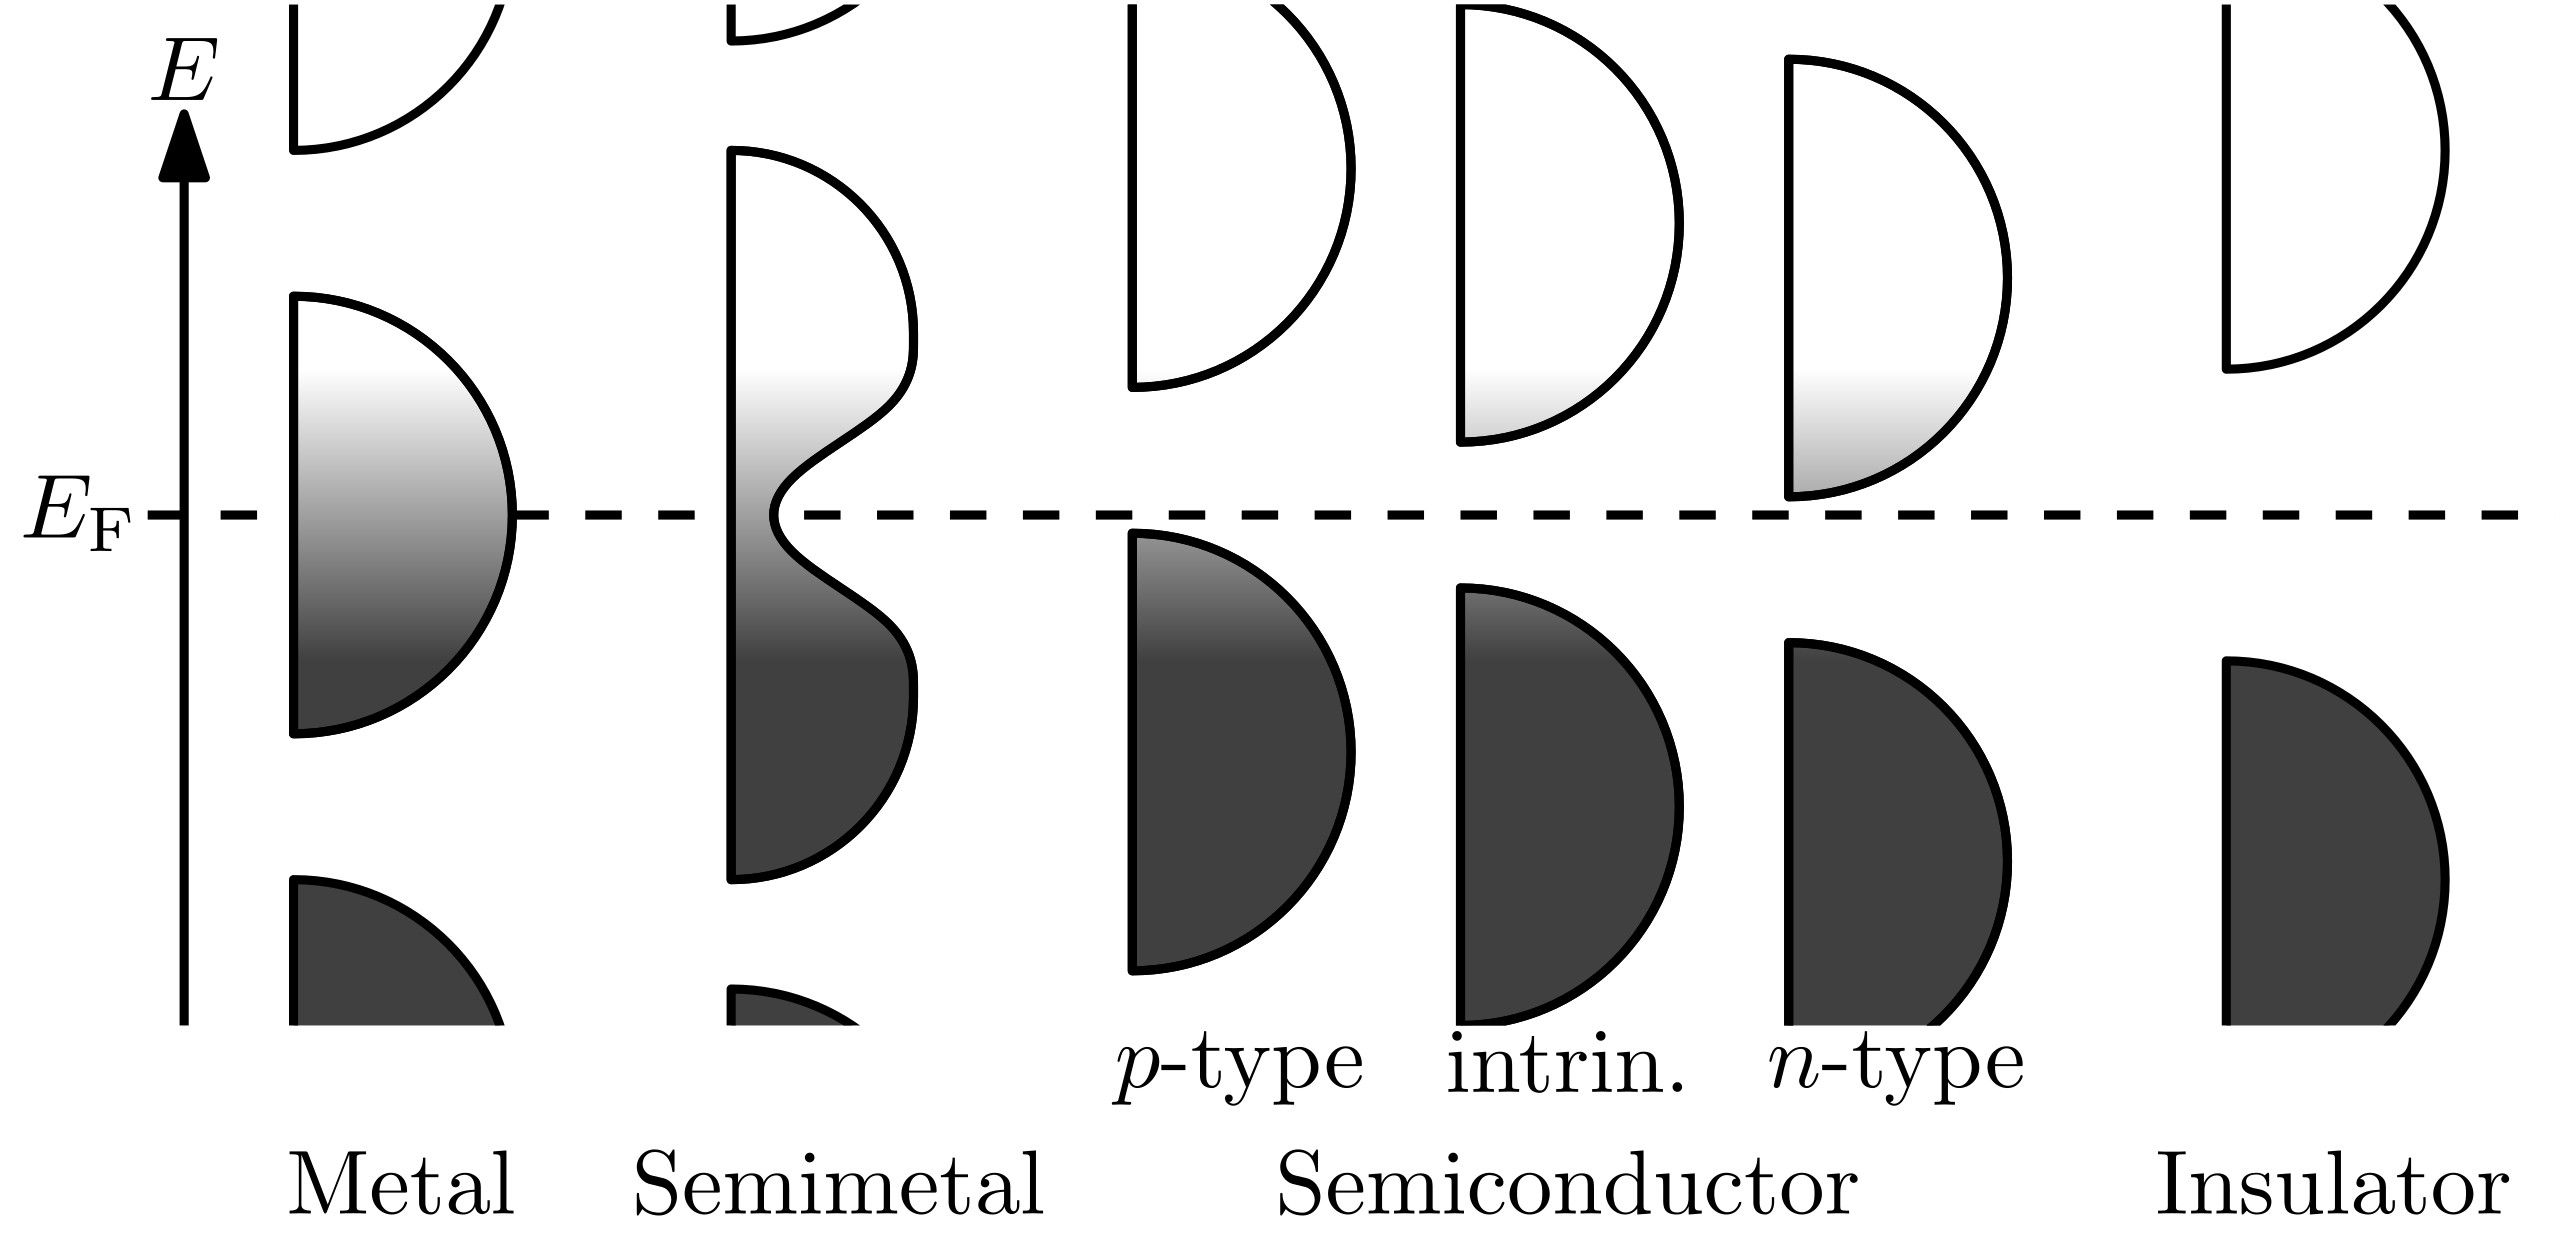
\includegraphics[scale = 0.08]{Figures/bi-magneto.png}
        \caption{Filling of the electronic states in various types of materials at equilibrium. Here, height is energy while width is the density of available states for a certain energy in the material listed. The shade follows the Fermi–Dirac distribution (black = all states filled, white = no state filled). In metals and semimetals the Fermi level EF lies inside at least one band. In insulators and semiconductors the Fermi level is inside a band gap; however, in semiconductors the bands are near enough to the Fermi level to be thermally populated with electrons or holes.}
        \label{fig:bimagneto}
    \end{figure}
    
\section{Observations}
    The Hall voltage reading corresponding to different magnetic field values at ambient temperature for Bi is tabulated in table (\ref{tab:bihall}), for p-Ge in table (\ref{tab:hallpGe}) and for n-Ge in table (\ref{tab:hallnGe}). The data of magneto-resistance for Bi is tabulated in table (\ref{tab:magBi}) and for n-Ge in table (\ref{tab:magGe}). The $V_h \sim H$ plots for Bi, p-Ge and n-Ge are given in figures (\ref{fig:hallbiplot}), (\ref{fig:hallpGeplot}) and (\ref{fig:hallnGeplot}) respectively. The $\Delta R/R \sim H$ plots for Bi and n-Ge are given in figures (\ref{fig:bimgst}) and (\ref{fig:nGemgrst}) respectively and their corresponding logarithmic plots are given in figures (\ref{fig:logbi}) and (\ref{fig:lognGe}) respectively. Additionally following observations were made:
    \begin{enumerate}
        \item Ambient temperature $T =23 \celsius$
        \item Probe current for Bi when studying Hall's effect $I= \SI{190}{\milli \ampere}$.
        \item Thickness of Bi sample when studying Hall's effect $z =\SI{0.5}{\milli \metre}$.
        \item Probe current for p-Ge when studying Hall's effect $I= \SI{0.98}{ \ampere}$.
        \item Thickness of p-Ge sample when studying Hall's effect $z =\SI{0.5}{\milli \metre}$.
        \item Probe current for n-Ge when studying Hall's effect $I = \SI{1.2}{ \ampere}$.
        \item Thickness of n-Ge sample when studying Hall's effect $z =\SI{0.5}{\milli \metre}$.
        \item Probe current for Bi when studying magneto-resistance $= \SI{195.8}{\milli \ampere}$.
        \item Resistance without magnetic field for Bi $R = \SI{7.5587e-4}{\ohm}$.
        \item Probe current for n-Ge when studying magneto-resistance $I = \SI{4}{\milli \ampere}$.
        \item Resistance without magnetic field for n-Ge $R = \SI{43.92}{\ohm}$.
        \item Resistivity of Bi $\rho = \SI{1.29e-4}{\ohm \centi \metre}$.
        \item Resistivity of p-Ge $\rho = \SI{1.29e-4}{\ohm \centi \metre}$.
    \end{enumerate}

% Please add the following required packages to your document preamble:
% \usepackage{booktabs}
\begin{table}[]
\caption{Variance of Hall voltage with magnetic field for Bi}
\label{tab:bihall}
\begin{tabular}{@{}cccc@{}}
\toprule
\textbf{\#} &
  \textbf{\begin{tabular}[c]{@{}c@{}}Current $I$\\ ($\si{\ampere}$)\end{tabular}} &
  \textbf{\begin{tabular}[c]{@{}c@{}}Magnetic field $H$\\ $(\si{\gauss})$\end{tabular}} &
  \textbf{\begin{tabular}[c]{@{}c@{}}Hall voltage $V_H$\\ ($\si{\milli \volt}$)\end{tabular}} \\ \midrule
1  & 0    & 0    & 0      \\
2  & 0.2  & 1106 & -0.004 \\
3  & 0.31 & 1556 & -0.008 \\
4  & 0.4  & 1997 & -0.01  \\
5  & 0.5  & 2490 & -0.013 \\
6  & 0.6  & 2910 & -0.016 \\
7  & 0.7  & 3370 & -0.018 \\
8  & 0.8  & 3890 & -0.02  \\
9  & 0.9  & 4320 & -0.022 \\
10 & 1    & 4770 & -0.024 \\
11 & 1.2  & 5610 & -0.028 \\
12 & 1.5  & 6790 & -0.032 \\
13 & 1.81 & 7680 & -0.035 \\
14 & 2.1  & 8340 & -0.037 \\
15 & 2.4  & 8840 & -0.038 \\
16 & 2.7  & 9240 & -0.04  \\
17 & 3    & 9590 & -0.041 \\ \bottomrule
\end{tabular}
\end{table}


% Please add the following required packages to your document preamble:
% \usepackage{booktabs}
\begin{table}[]
\caption{Variance of Hall voltage with magnetic field for p-Ge}
\label{tab:hallpGe}
\begin{tabular}{@{}cccc@{}}
\toprule
\textbf{\#} &
  \textbf{\begin{tabular}[c]{@{}c@{}}Current $I$\\ ($\si{\ampere}$)\end{tabular}} &
  \textbf{\begin{tabular}[c]{@{}c@{}}Magnetic field $H$\\ $(\si{\gauss})$\end{tabular}} &
  \textbf{\begin{tabular}[c]{@{}c@{}}Hall voltage $V_H$\\ ($\si{\milli \volt}$)\end{tabular}} \\ \midrule
1  & 0.01 & 9.669    & 1.5  \\
2  & 0.15 & 145.035  & 2.2  \\
3  & 0.25 & 241.725  & 2.7  \\
4  & 0.35 & 338.415  & 3.2  \\
5  & 0.45 & 435.105  & 3.7  \\
6  & 0.55 & 531.795  & 4.2  \\
7  & 0.65 & 628.485  & 4.8  \\
8  & 0.75 & 725.175  & 5.3  \\
9  & 0.87 & 841.203  & 5.9  \\
10 & 0.95 & 918.555  & 6.3  \\
11 & 1.01 & 976.569  & 6.7  \\
12 & 1.15 & 1111.935 & 7.4  \\
13 & 1.25 & 1208.625 & 7.9  \\
14 & 1.35 & 1305.315 & 8.4  \\
15 & 1.45 & 1402.005 & 8.9  \\
16 & 1.55 & 1498.695 & 9.4  \\
17 & 1.66 & 1605.054 & 9.9  \\
18 & 1.77 & 1711.413 & 10.4 \\
19 & 1.86 & 1798.434 & 10.8 \\
20 & 1.95 & 1885.455 & 11.2 \\
21 & 2    & 1933.8   & 11.5 \\
22 & 2.15 & 2078.835 & 12.1 \\
23 & 2.25 & 2175.525 & 12.6 \\
24 & 2.35 & 2272.215 & 13   \\
25 & 2.45 & 2368.905 & 13.4 \\
26 & 2.55 & 2465.595 & 13.8 \\
27 & 2.65 & 2562.285 & 14.2 \\
28 & 2.75 & 2658.975 & 14.6 \\
29 & 2.86 & 2765.334 & 15   \\
30 & 2.95 & 2852.355 & 15.4 \\
31 & 3.01 & 2910.369 & 15.6 \\
32 & 3.15 & 3045.735 & 16.1 \\
33 & 3.26 & 3152.094 & 16.5 \\
34 & 3.35 & 3239.115 & 16.8 \\
35 & 3.45 & 3335.805 & 17.1 \\
36 & 3.57 & 3451.833 & 17.5 \\
37 & 3.65 & 3529.185 & 17.8 \\
38 & 3.76 & 3635.544 & 18.1 \\
39 & 3.88 & 3751.572 & 18.5 \\
40 & 3.96 & 3828.924 & 18.7 \\
41 & 4.02 & 3886.938 & 18.9 \\
42 & 4.1  & 3964.29  & 19.1 \\ \bottomrule
\end{tabular}
\end{table}


% Please add the following required packages to your document preamble:
% \usepackage{booktabs}
\begin{table}[]
\caption{Variance of Hall voltage with magnetic field for n-Ge}
\label{tab:hallnGe}
\begin{tabular}{@{}cccc@{}}
\toprule
\textbf{S.no} &
  \textbf{\begin{tabular}[c]{@{}c@{}}Current $I$\\ ($\si{\ampere}$)\end{tabular}} &
  \textbf{\begin{tabular}[c]{@{}c@{}}Magnetic field $H$\\ $(\si{\gauss})$\end{tabular}} &
  \textbf{\begin{tabular}[c]{@{}c@{}}Hall voltage $V_H$\\ ($\si{\milli \volt}$)\end{tabular}} \\ \midrule
1  & 0.15 & 145.035  & -2.1  \\
2  & 0.28 & 270.732  & -3.2  \\
3  & 0.36 & 348.084  & -4    \\
4  & 0.46 & 444.774  & -4.9  \\
5  & 0.55 & 531.795  & -5.9  \\
6  & 0.66 & 638.154  & -6.9  \\
7  & 0.75 & 725.175  & -7.7  \\
8  & 0.85 & 821.865  & -8.6  \\
9  & 0.96 & 928.224  & -9.7  \\
10 & 1.02 & 986.238  & -10.2 \\
11 & 1.16 & 1121.604 & -11.6 \\
12 & 1.25 & 1208.625 & -12.5 \\
13 & 1.35 & 1305.315 & -13.4 \\
14 & 1.45 & 1402.005 & -14.4 \\
15 & 1.56 & 1508.364 & -15.4 \\
16 & 1.66 & 1605.054 & -16.4 \\
17 & 1.76 & 1701.744 & -17.3 \\
18 & 1.85 & 1788.765 & -18.1 \\
19 & 1.96 & 1895.124 & -19.1 \\
20 & 2.01 & 1943.469 & -19.6 \\
21 & 2.15 & 2078.835 & -20.9 \\
22 & 2.25 & 2175.525 & -21.9 \\
23 & 2.36 & 2281.884 & -22.8 \\
24 & 2.47 & 2388.243 & -23.8 \\
25 & 2.55 & 2465.595 & -24.6 \\
26 & 2.65 & 2562.285 & -25.4 \\
27 & 2.75 & 2658.975 & -26.3 \\
28 & 2.85 & 2755.665 & -27.2 \\
29 & 2.95 & 2852.355 & -28.1 \\
30 & 3.02 & 2920.038 & -28.7 \\
31 & 3.15 & 3045.735 & -29.7 \\
32 & 3.26 & 3152.094 & -30.7 \\
33 & 3.36 & 3248.784 & -31.5 \\
34 & 3.5  & 3384.15  & -32.7 \\
35 & 3.63 & 3509.847 & -33.8 \\
36 & 3.76 & 3635.544 & -34.7 \\
37 & 3.85 & 3722.565 & -35.5 \\
38 & 3.95 & 3819.255 & -36.1 \\
39 & 4.12 & 3983.628 & -37.3 \\ \bottomrule
\end{tabular}
\end{table}
% Please add the following required packages to your document preamble:
% \usepackage{booktabs}
\begin{table}[]
\caption{Data for magneto-resistance for Bi}
\label{tab:magBi}
\begin{tabular}{@{}ccccccc@{}}
\toprule
\textbf{\#} &
  \textbf{\begin{tabular}[c]{@{}c@{}}Magnetic \\ field $H$ \\ ($\si{\kilo \gauss}$)\end{tabular}} &
  \textbf{\begin{tabular}[c]{@{}c@{}}Voltage \\ ($\si{\milli \volt}$)\end{tabular}} &
  \textbf{\begin{tabular}[c]{@{}c@{}}$R_m$ \\ ($\si{\milli \ohm}$)\end{tabular}} &
  \textbf{\begin{tabular}[c]{@{}c@{}}$\Delta R/R$ \\ ($10^{-3}$)\end{tabular}} &
  \textbf{\begin{tabular}[c]{@{}c@{}}$\log H$ \\ ($\si{\gauss}$)\end{tabular}} &
  \textbf{\begin{tabular}[c]{@{}c@{}}$\log$ ($\Delta R/R$) \\ ($10^{-3}$)\end{tabular}} \\ \midrule
1  & 0.5403 & 0.149 & 0.761 & 6.761   & 2.733 & 0.830 \\
2  & 1.0336 & 0.151 & 0.771 & 20.275  & 3.014 & 1.307 \\
3  & 1.3859 & 0.152 & 0.776 & 27.032  & 3.142 & 1.432 \\
4  & 1.7617 & 0.153 & 0.781 & 33.788  & 3.246 & 1.529 \\
5  & 1.9966 & 0.154 & 0.787 & 40.545  & 3.300 & 1.608 \\
6  & 2.5134 & 0.156 & 0.797 & 54.059  & 3.400 & 1.733 \\
7  & 2.9597 & 0.161 & 0.822 & 87.843  & 3.471 & 1.944 \\
8  & 3.2886 & 0.163 & 0.832 & 101.356 & 3.517 & 2.006 \\
9  & 3.4765 & 0.165 & 0.843 & 114.870 & 3.541 & 2.060 \\
10 & 3.8054 & 0.168 & 0.858 & 135.140 & 3.580 & 2.131 \\
11 & 4.1107 & 0.17  & 0.868 & 148.654 & 3.614 & 2.172 \\
12 & 4.3691 & 0.172 & 0.878 & 162.167 & 3.640 & 2.210 \\
13 & 4.651  & 0.174 & 0.889 & 175.681 & 3.668 & 2.245 \\
14 & 5.0973 & 0.175 & 0.894 & 182.438 & 3.707 & 2.261 \\
15 & 5.4497 & 0.176 & 0.899 & 189.194 & 3.736 & 2.277 \\
16 & 5.7785 & 0.178 & 0.909 & 202.708 & 3.762 & 2.307 \\
17 & 5.896  & 0.179 & 0.914 & 209.465 & 3.771 & 2.321 \\
18 & 6.0134 & 0.181 & 0.924 & 222.978 & 3.779 & 2.348 \\
19 & 6.0604 & 0.182 & 0.930 & 229.735 & 3.783 & 2.361 \\ \bottomrule
\end{tabular}
\end{table}

% Please add the following required packages to your document preamble:
% \usepackage{booktabs}
\begin{table}[]
\caption{Data for magneto-resistance for n-Ge}
\label{tab:magGe}
\begin{tabular}{@{}ccccccc@{}}
\toprule
\textbf{\#} &
  \textbf{\begin{tabular}[c]{@{}c@{}}Magnetic \\ field $H$ \\ ($\si{\kilo \gauss}$)\end{tabular}} &
  \textbf{\begin{tabular}[c]{@{}c@{}}Voltage \\ ($\si{\milli \volt}$)\end{tabular}} &
  \textbf{\begin{tabular}[c]{@{}c@{}}$R_m$ \\ ($\si{\milli \ohm}$)\end{tabular}} &
  \textbf{\begin{tabular}[c]{@{}c@{}}$\Delta R/R$ \\ ($10^{-3}$)\end{tabular}} &
  \textbf{\begin{tabular}[c]{@{}c@{}}$\log H$ \\ ($\si{\gauss}$)\end{tabular}} &
  \textbf{\begin{tabular}[c]{@{}c@{}}$\log$ ($\Delta R/R$) \\ ($10^{-3}$)\end{tabular}} \\ \midrule
1 & 0.793 & 175.9 & 43.975 & 1.252  & 2.899 & 0.098 \\
2 & 1.035 & 176.1 & 44.025 & 2.391  & 3.015 & 0.379 \\
3 & 1.29  & 176.3 & 44.075 & 3.529  & 3.111 & 0.548 \\
4 & 1.544 & 176.6 & 44.150 & 5.237  & 3.189 & 0.719 \\
5 & 2.05  & 177.2 & 44.300 & 8.652  & 3.312 & 0.937 \\
6 & 2.55  & 178   & 44.500 & 13.206 & 3.407 & 1.121 \\
7 & 3.05  & 178.9 & 44.725 & 18.329 & 3.484 & 1.263 \\
8 & 3.53  & 179.9 & 44.975 & 24.021 & 3.548 & 1.381 \\
9 & 4     & 180.9 & 45.225 & 29.713 & 3.602 & 1.473 \\ \bottomrule
\end{tabular}
\end{table}

\begin{figure}
    \centering
    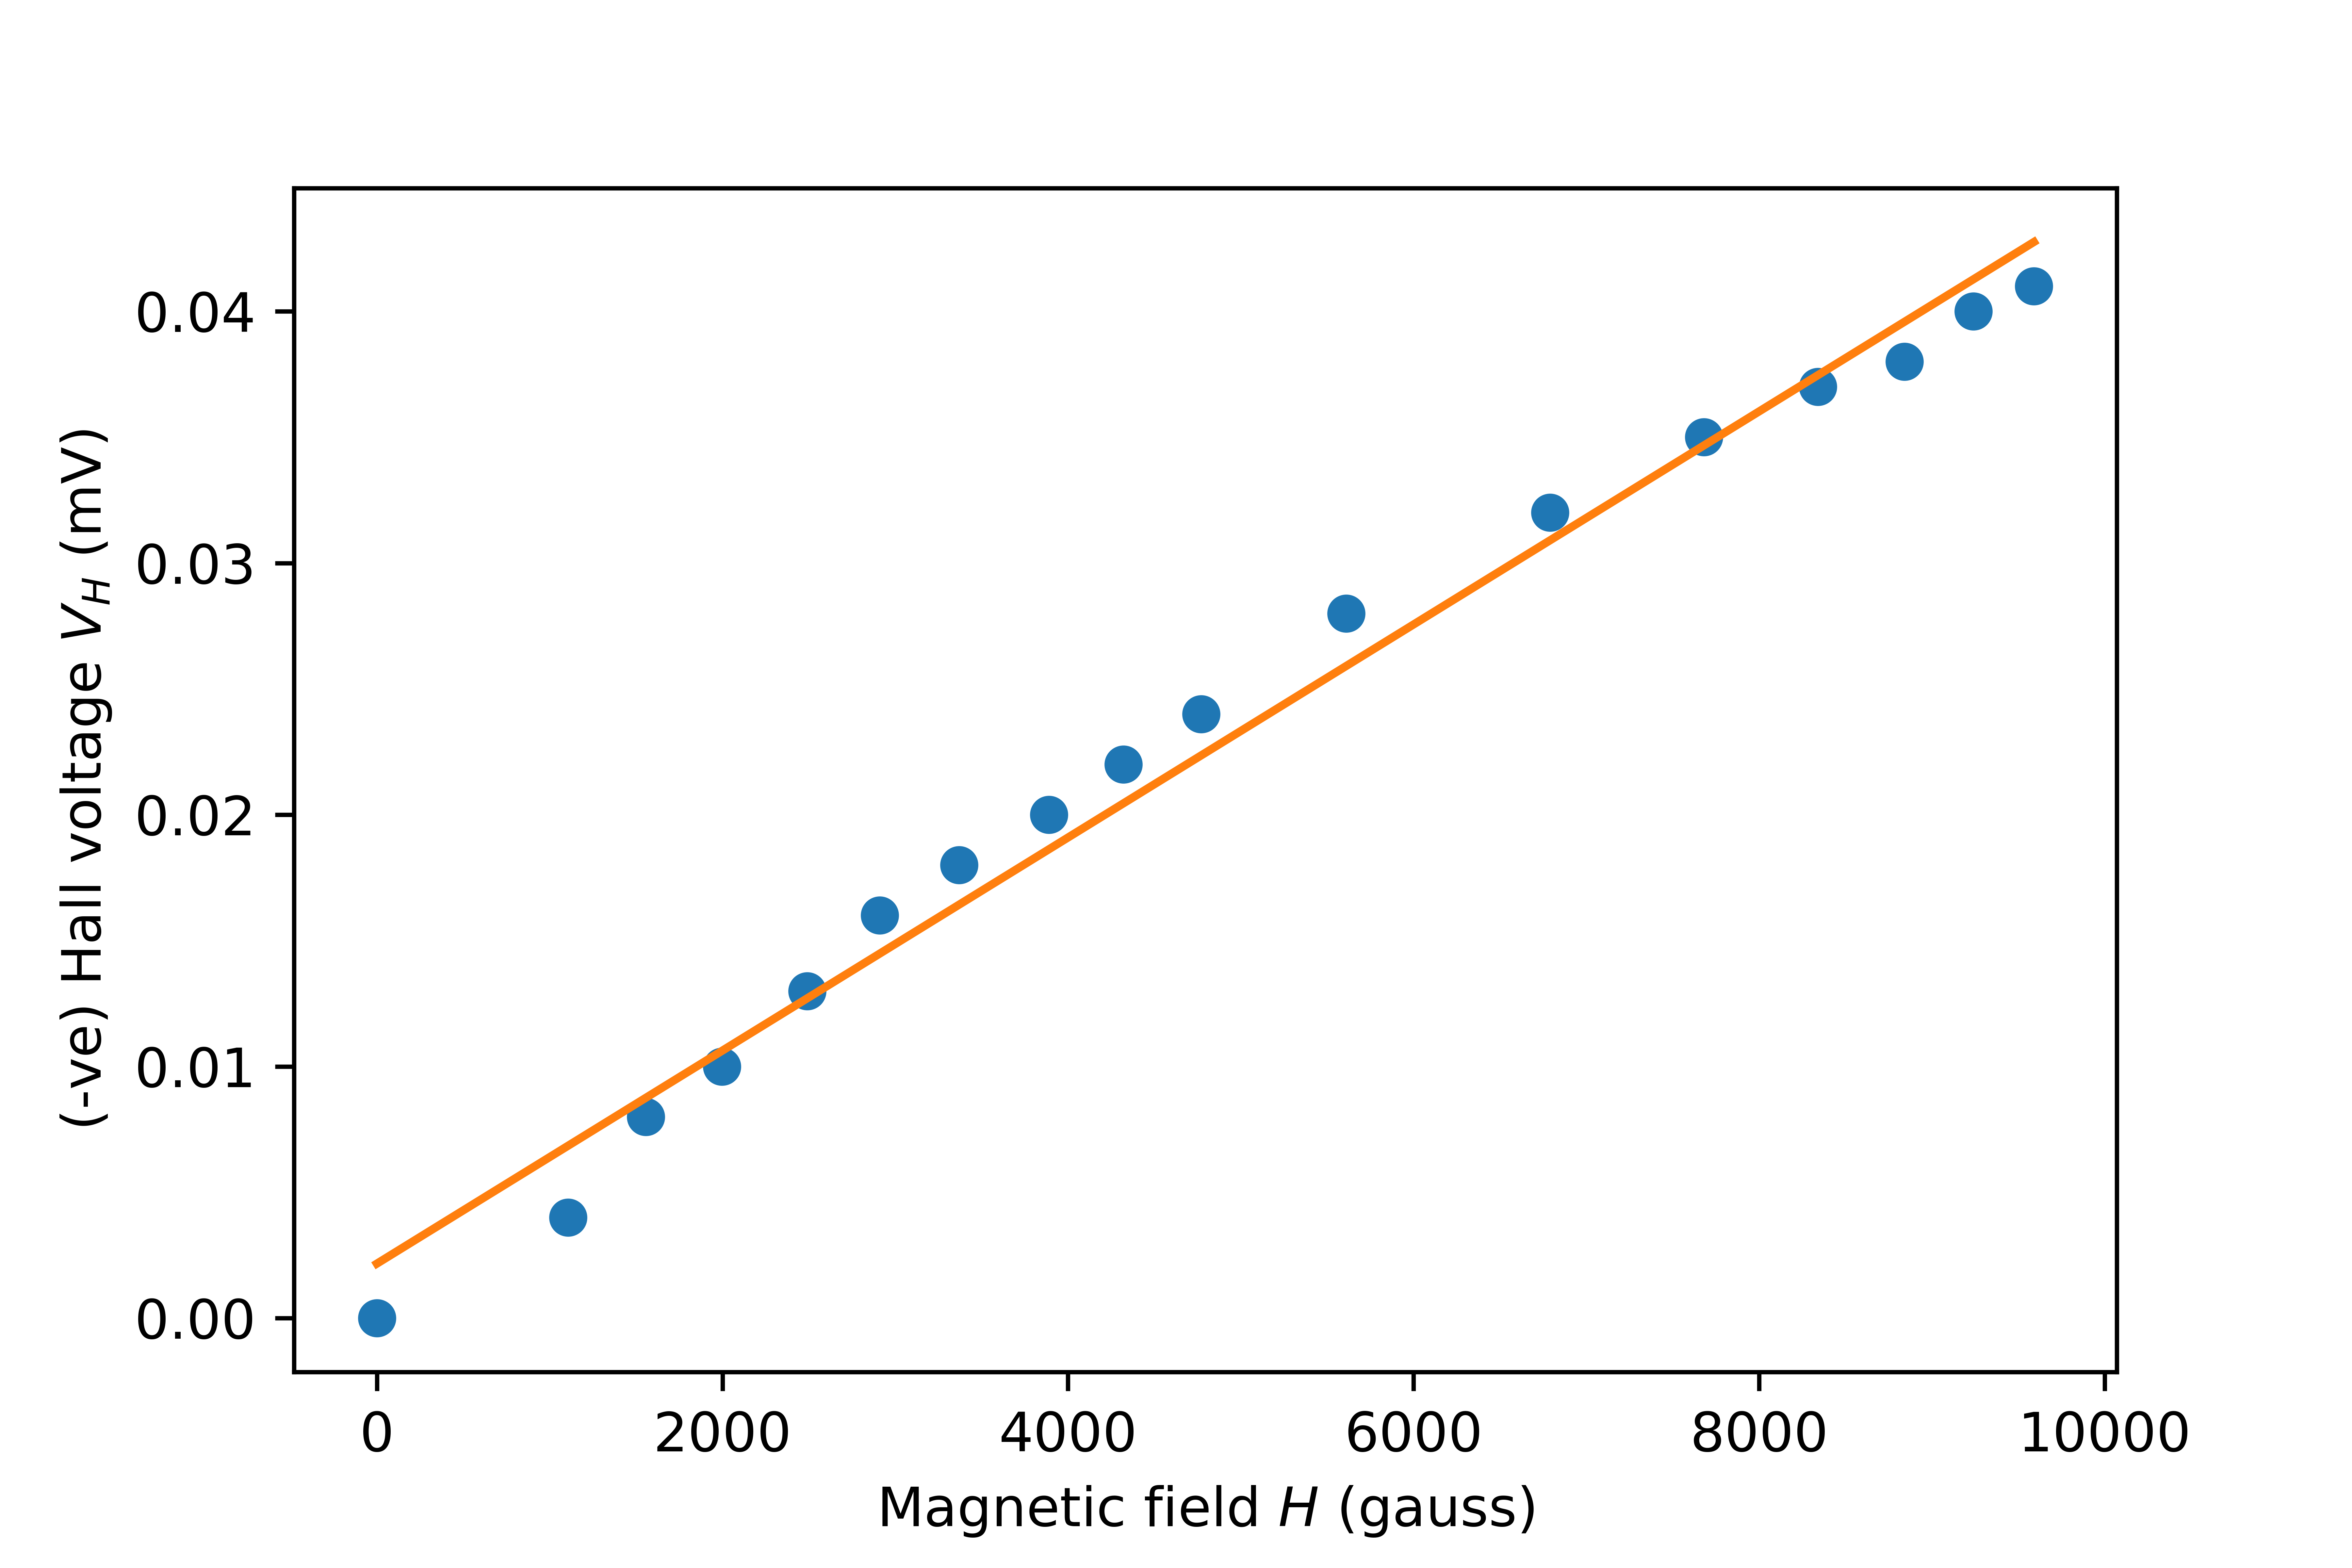
\includegraphics[scale = 0.56]{Figures/plot-hall-Bi.png}
    \caption{$V_h \sim H$ plot for Bi}
    \label{fig:hallbiplot}
\end{figure}
\begin{figure}
    \centering
    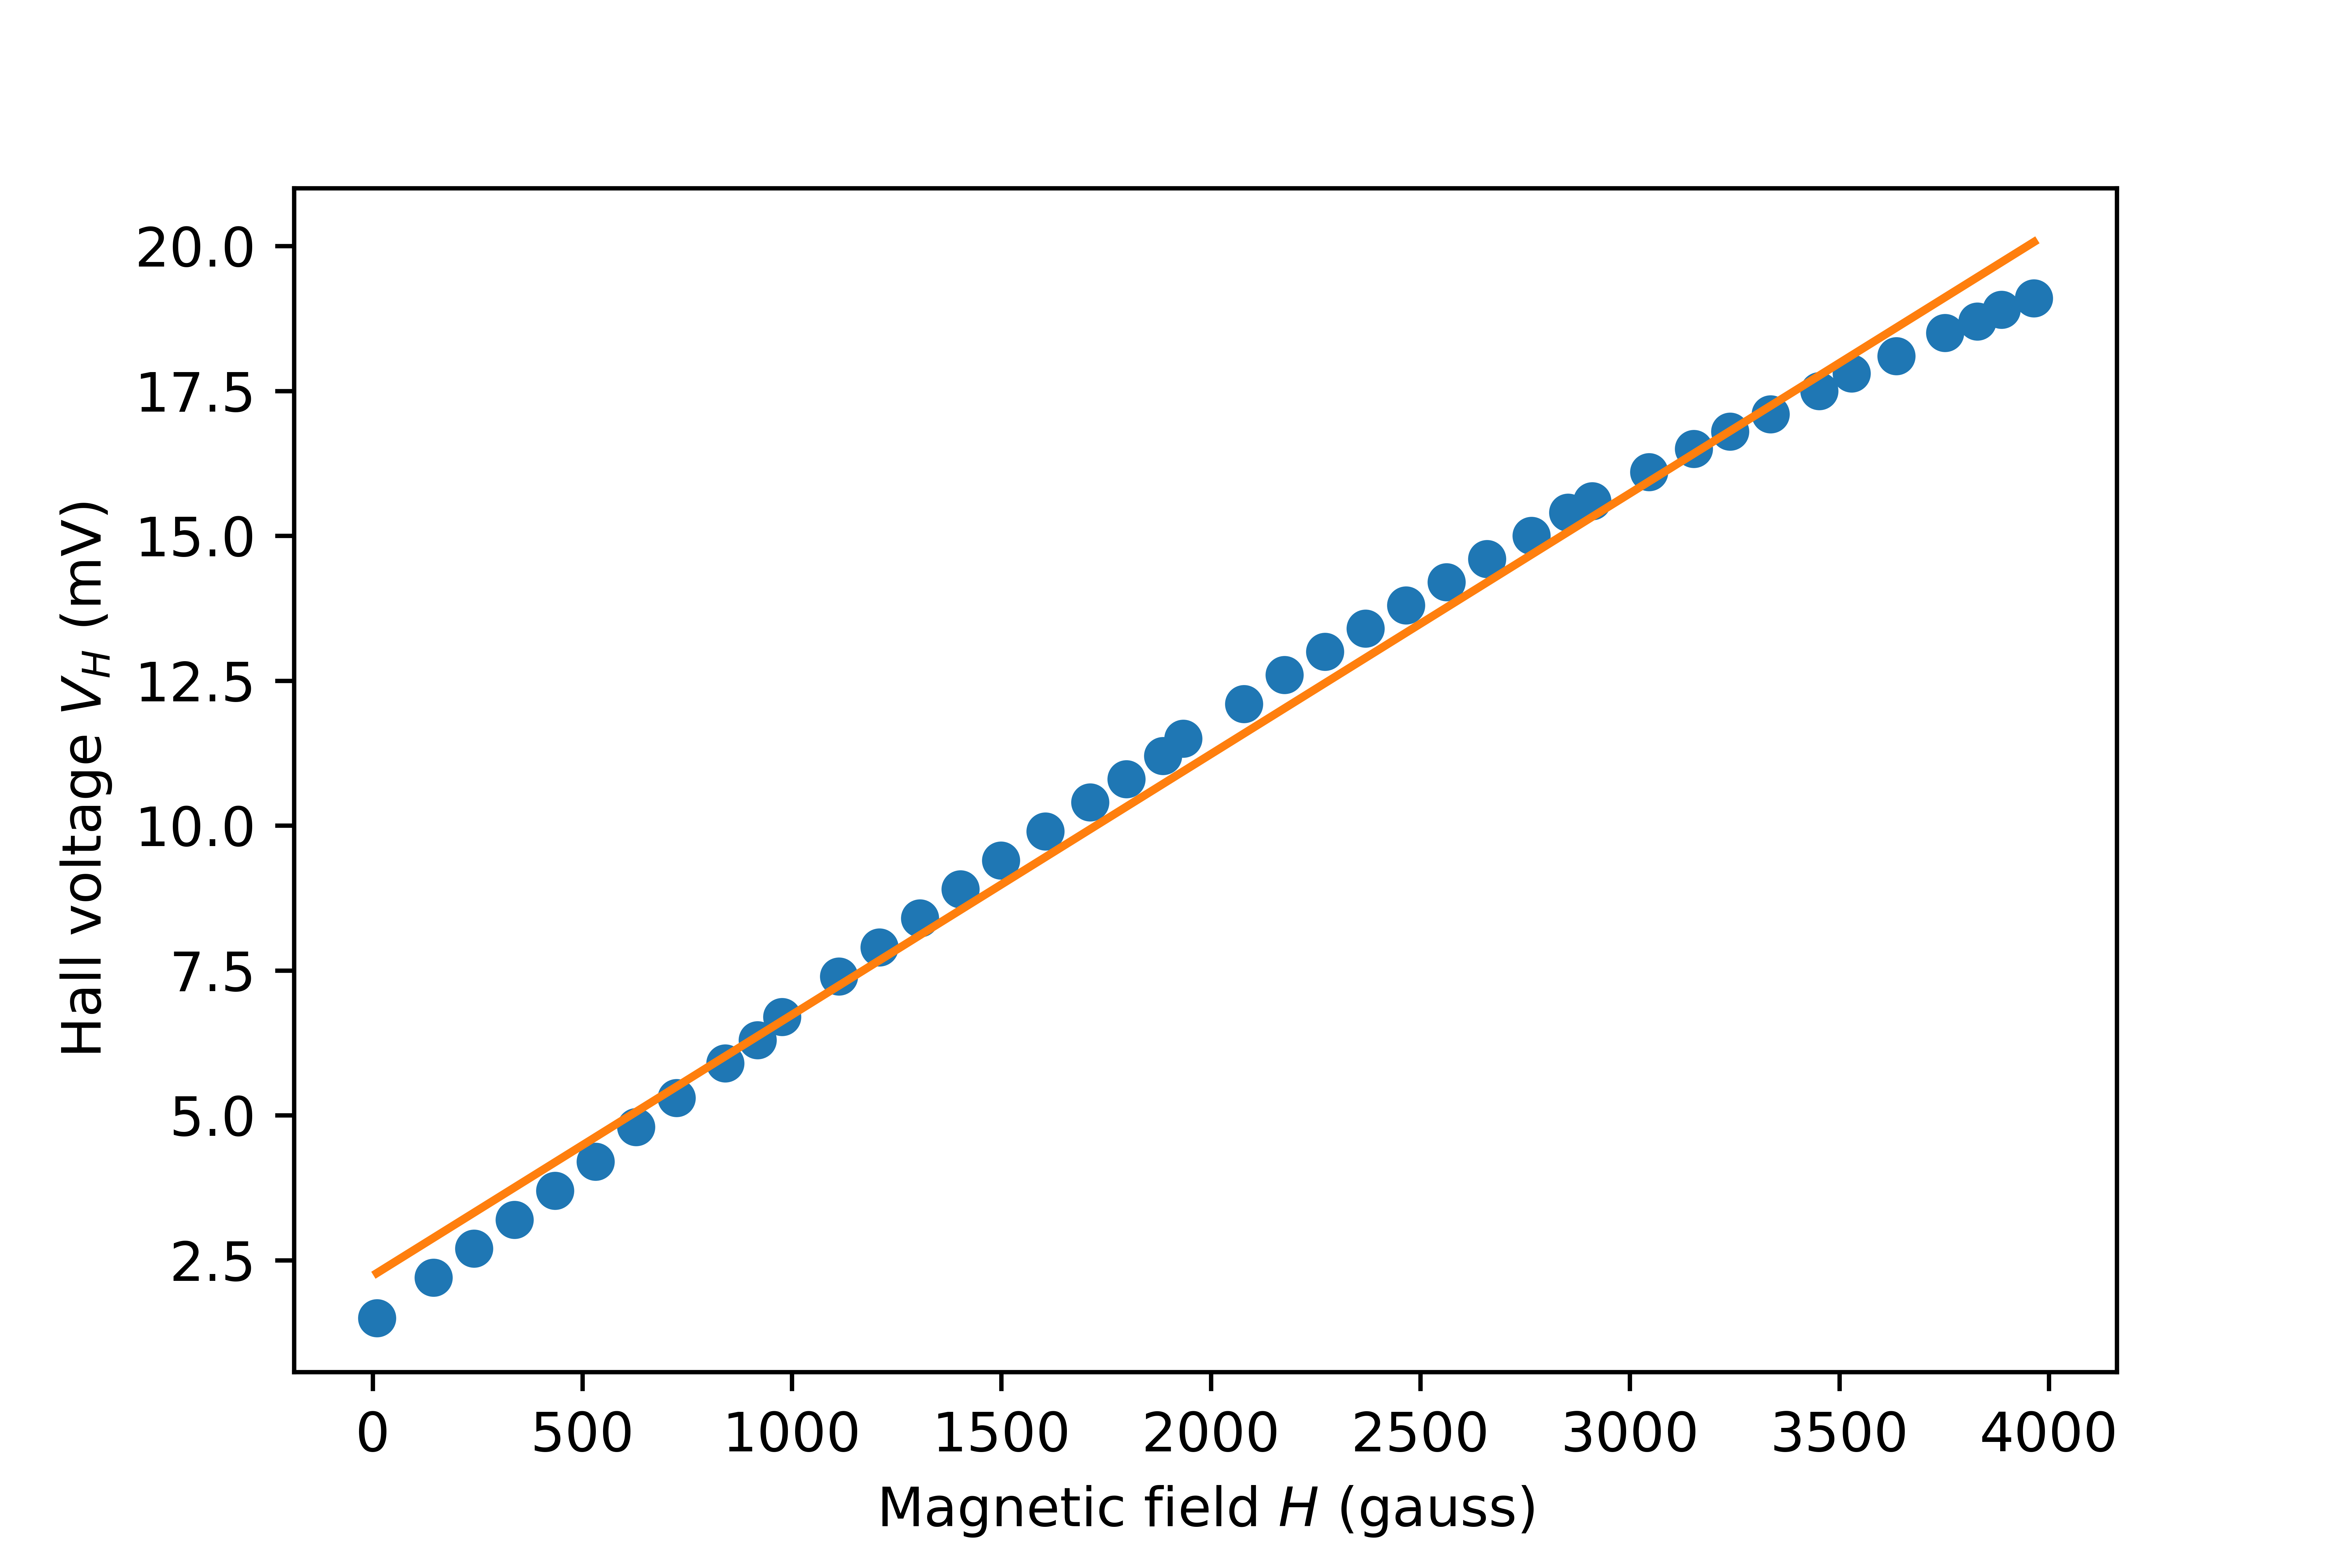
\includegraphics[scale = 0.56]{Figures/plot-hall-p-Ge.png}
    \caption{$V_h \sim H$ plot for p-Ge}
    \label{fig:hallpGeplot}
\end{figure}
\begin{figure}
    \centering
    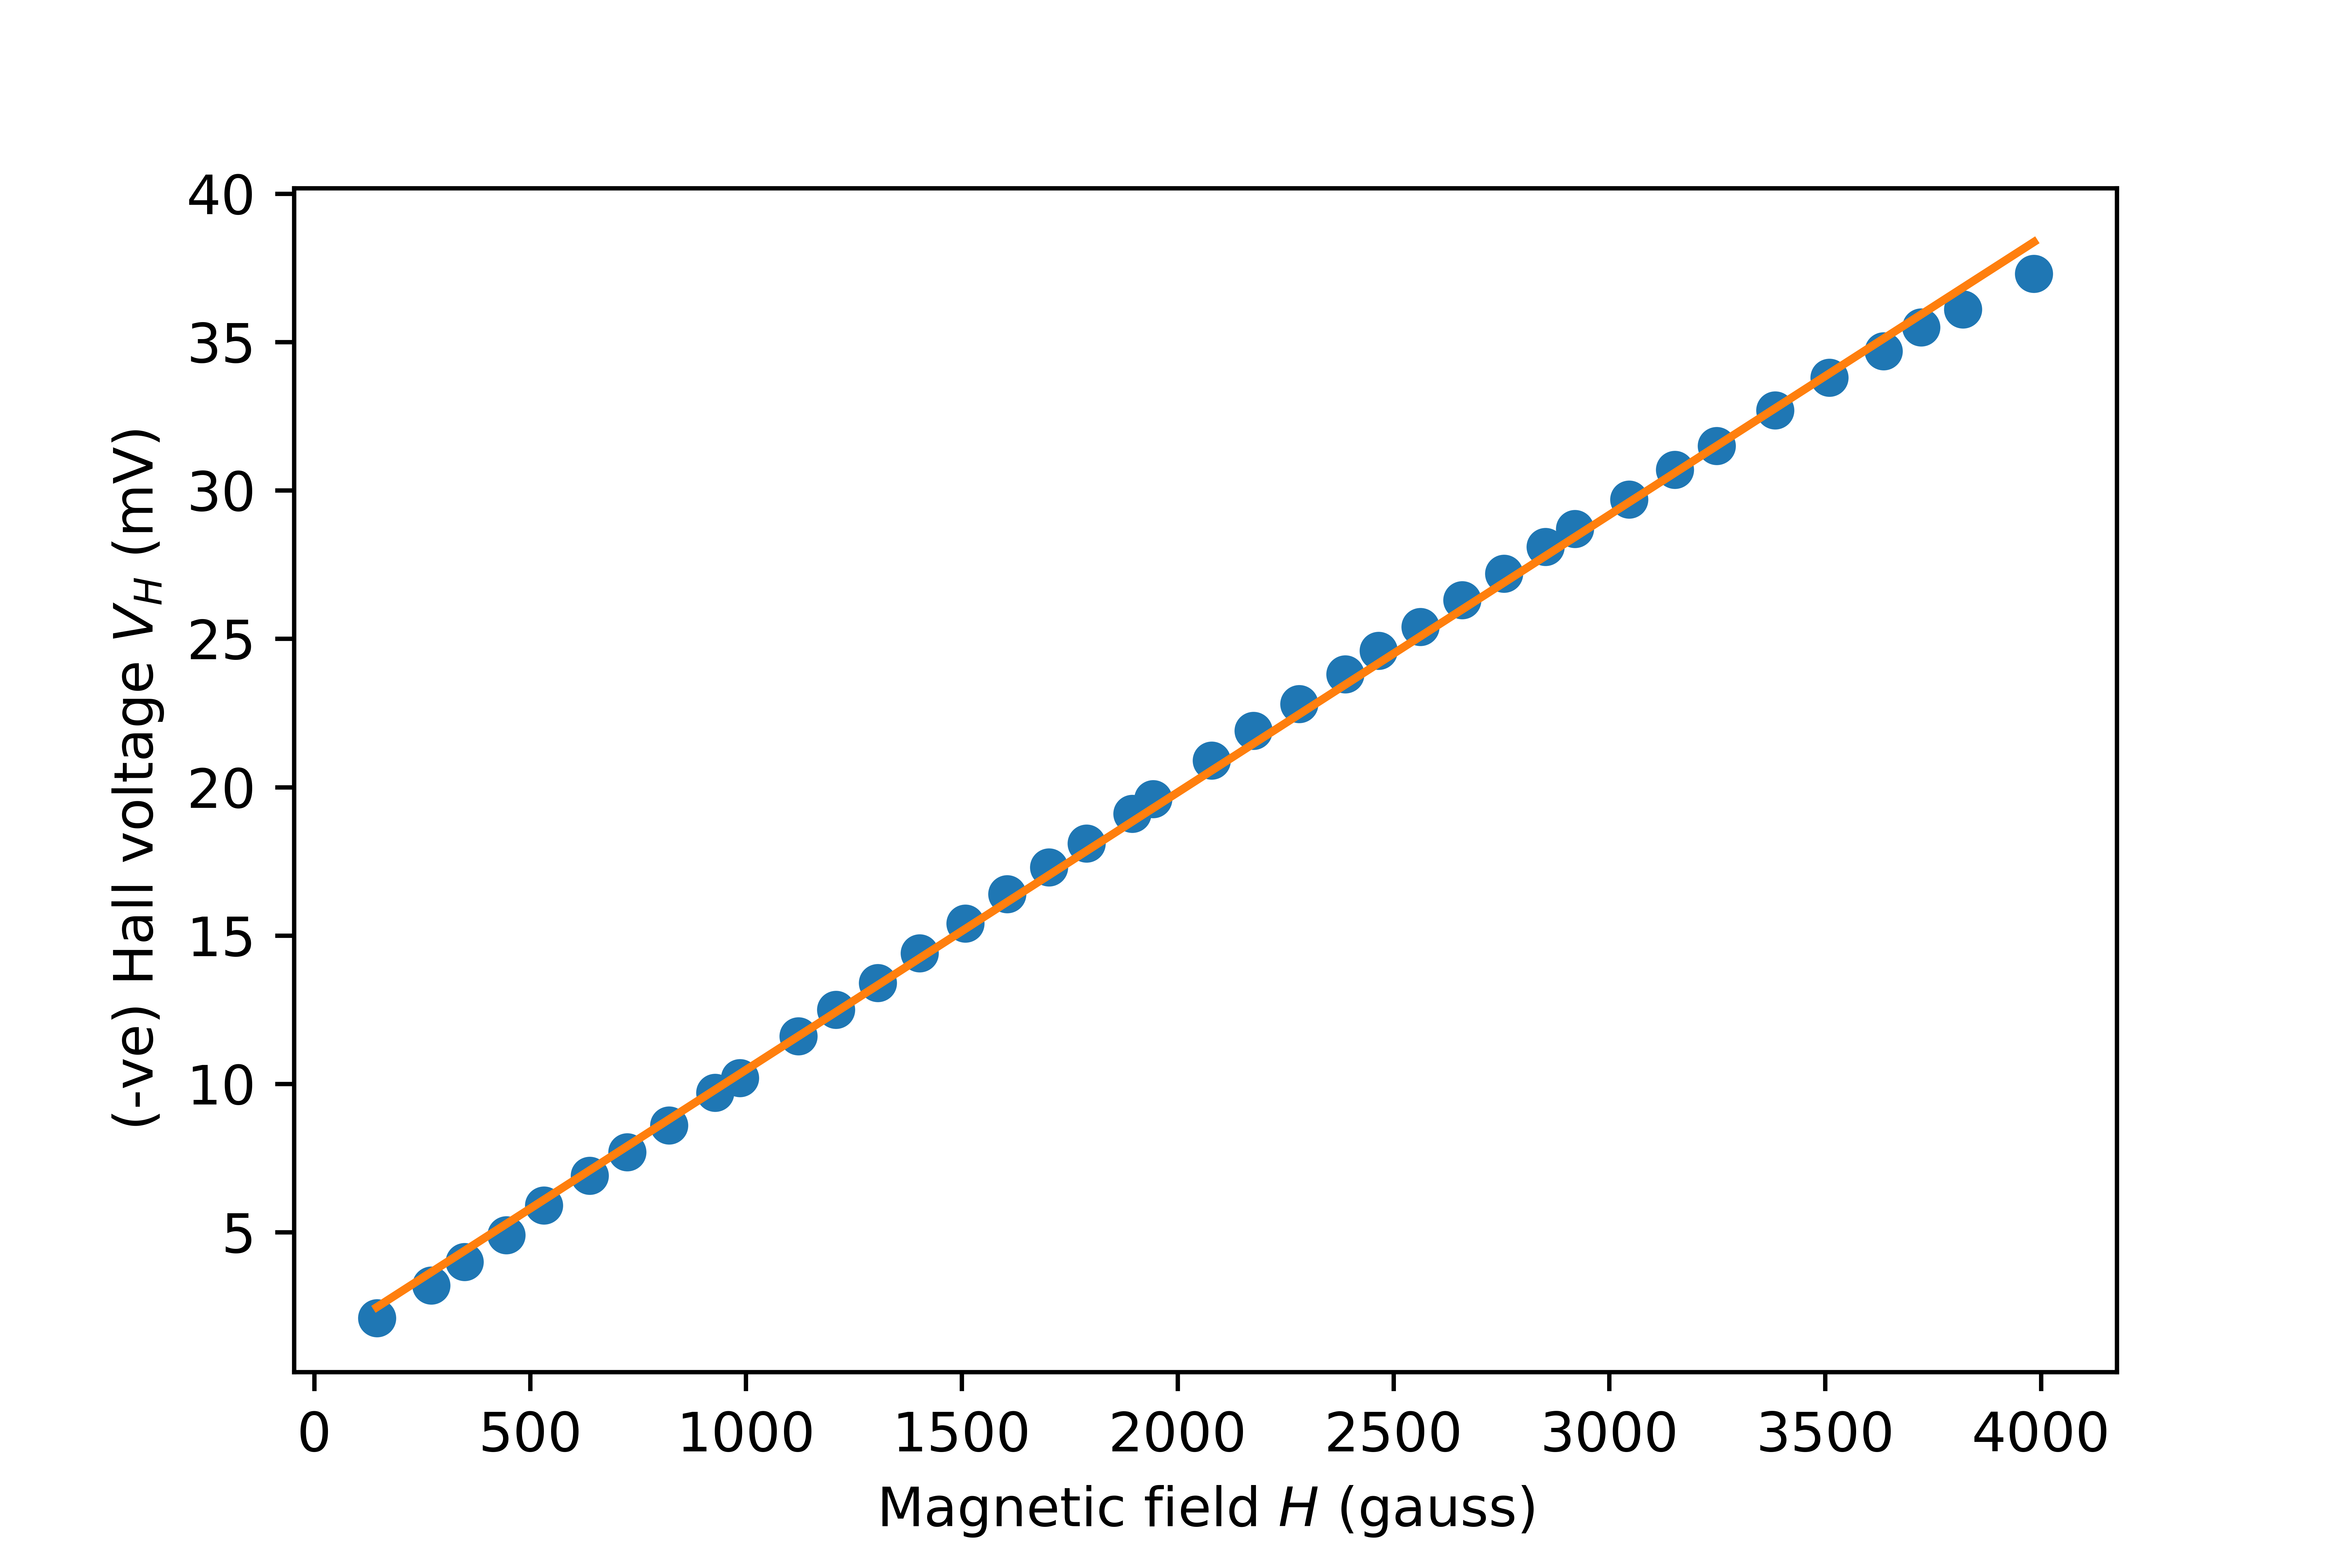
\includegraphics[scale = 0.56]{Figures/plot-hall-n-Ge.png}
    \caption{$V_h \sim H$ plot for n-Ge}
    \label{fig:hallnGeplot}
\end{figure}
\begin{figure}
    \centering
    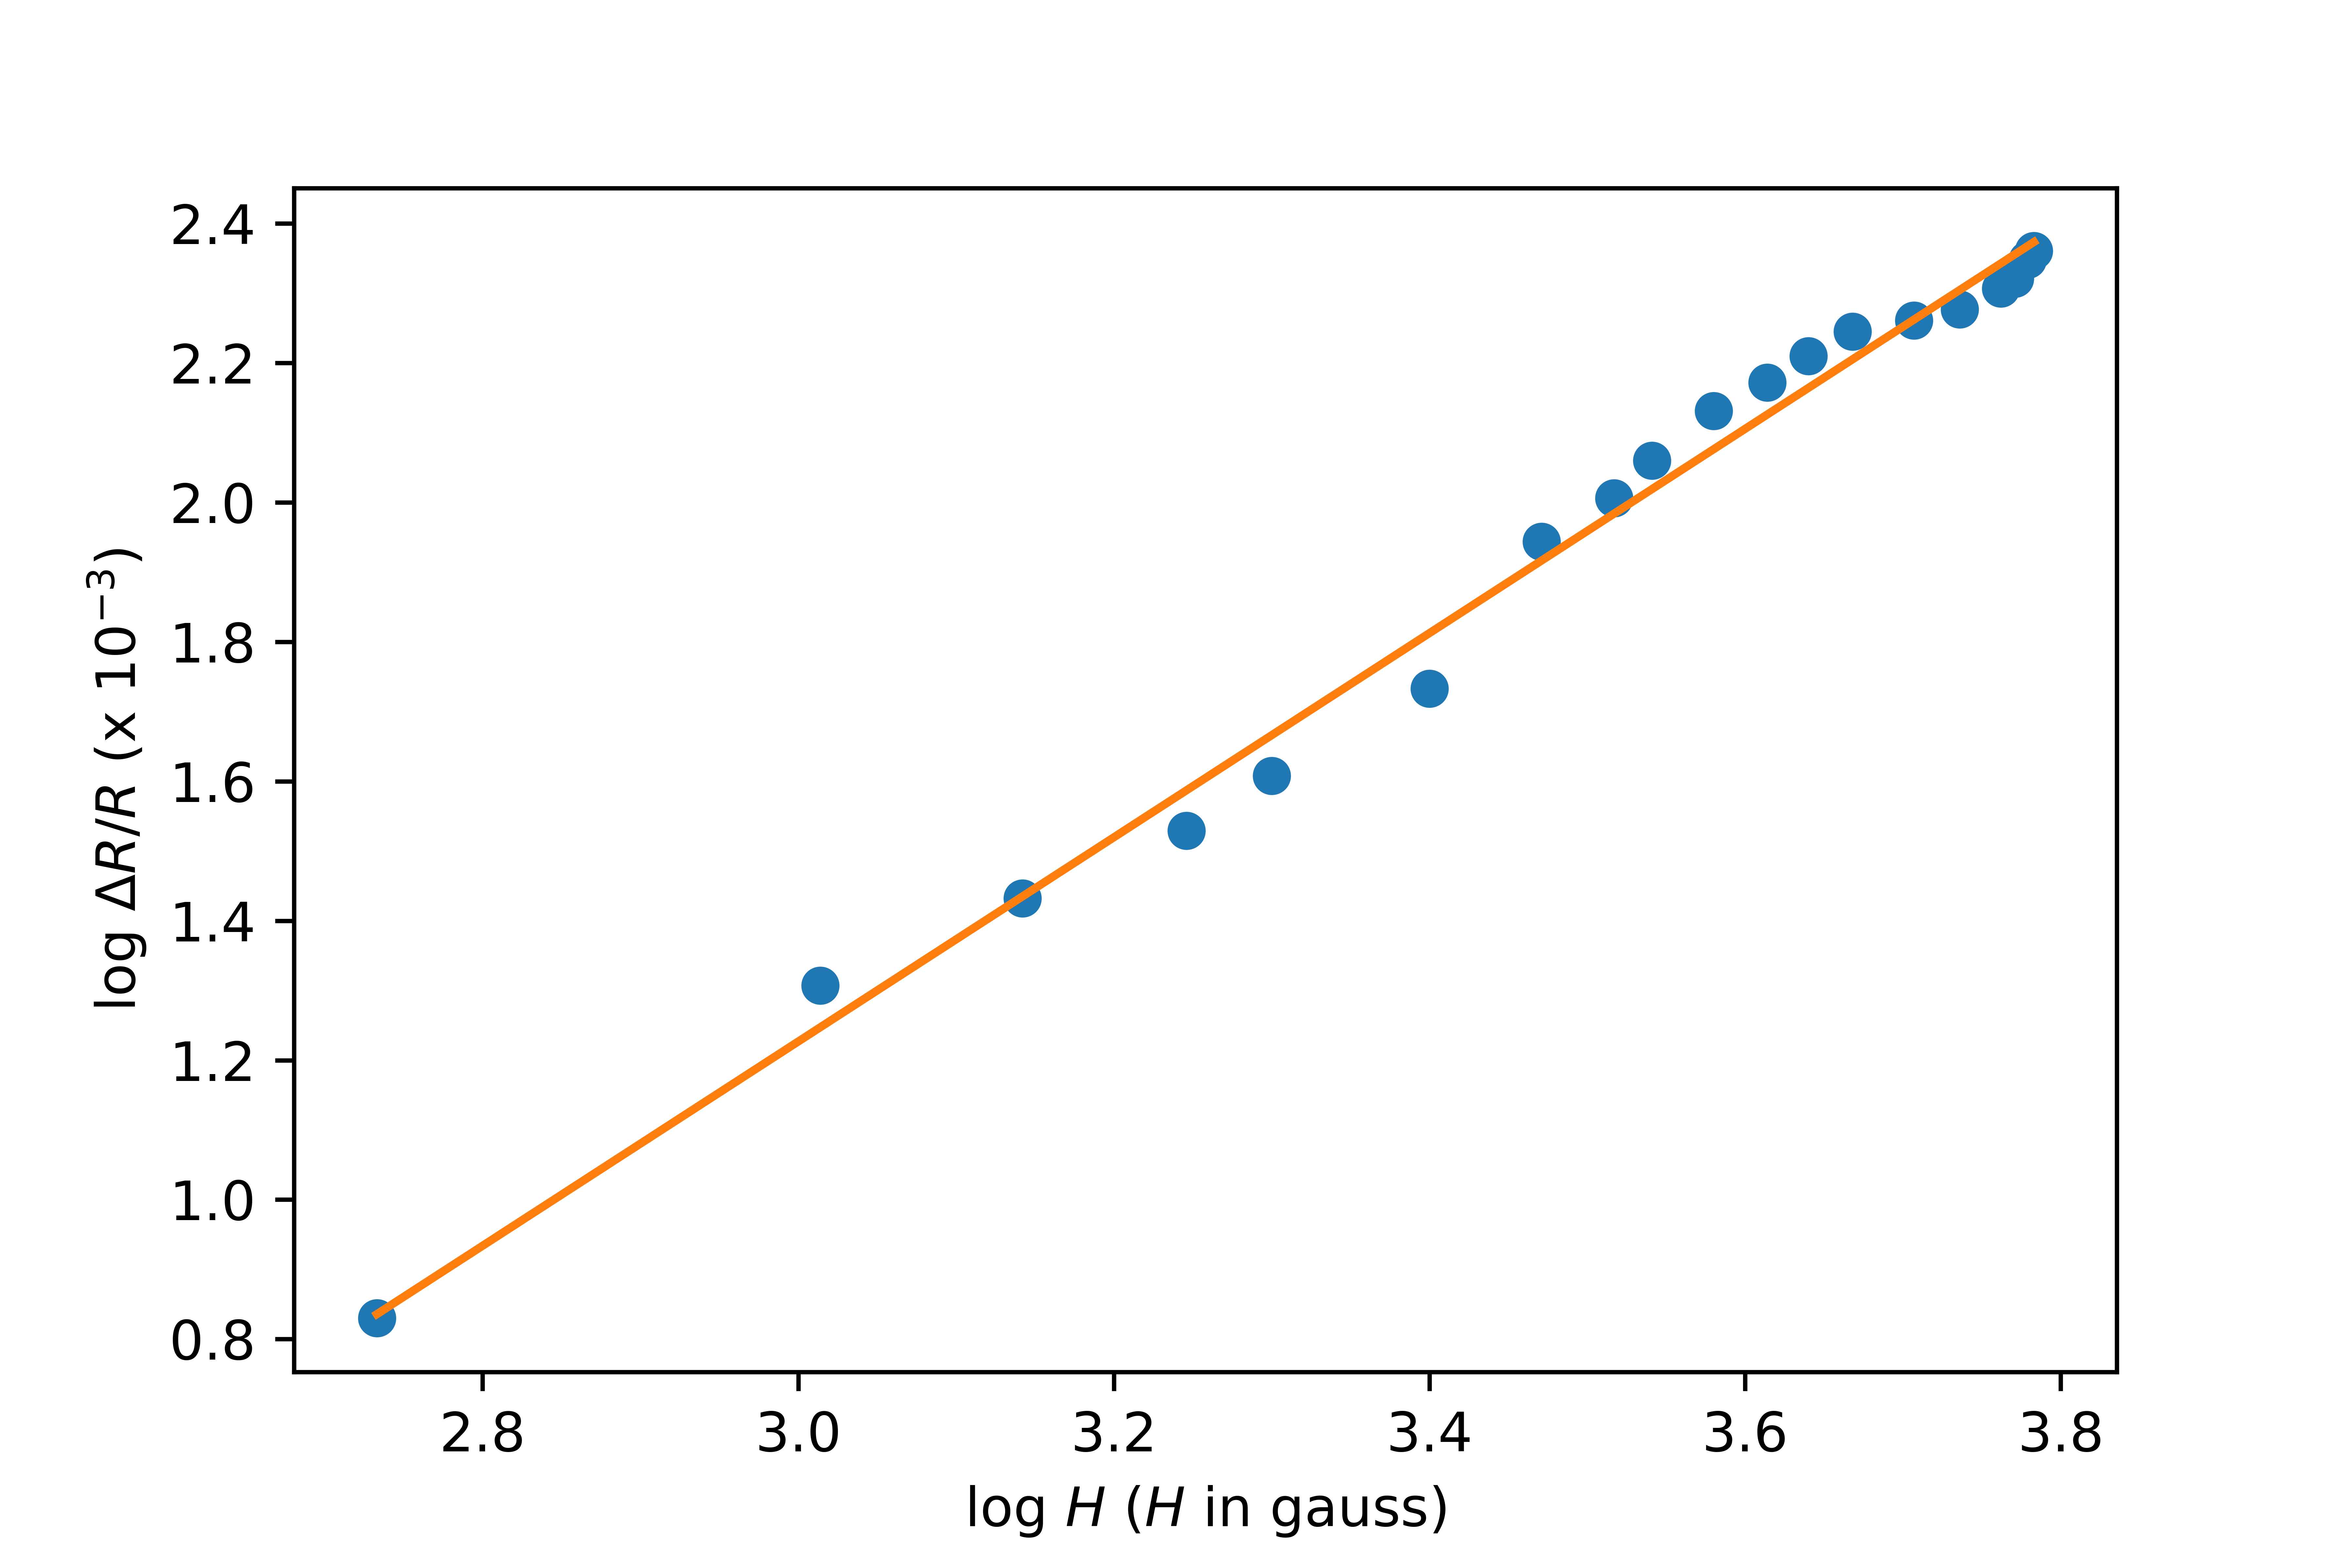
\includegraphics[scale = 0.56]{Figures/plot-mgrst-Bi-log.png}
    \caption{$\log \Delta R/R \sim \log H$ plot for Bi}
    \label{fig:logbi}
\end{figure}
\begin{figure}
    \centering
    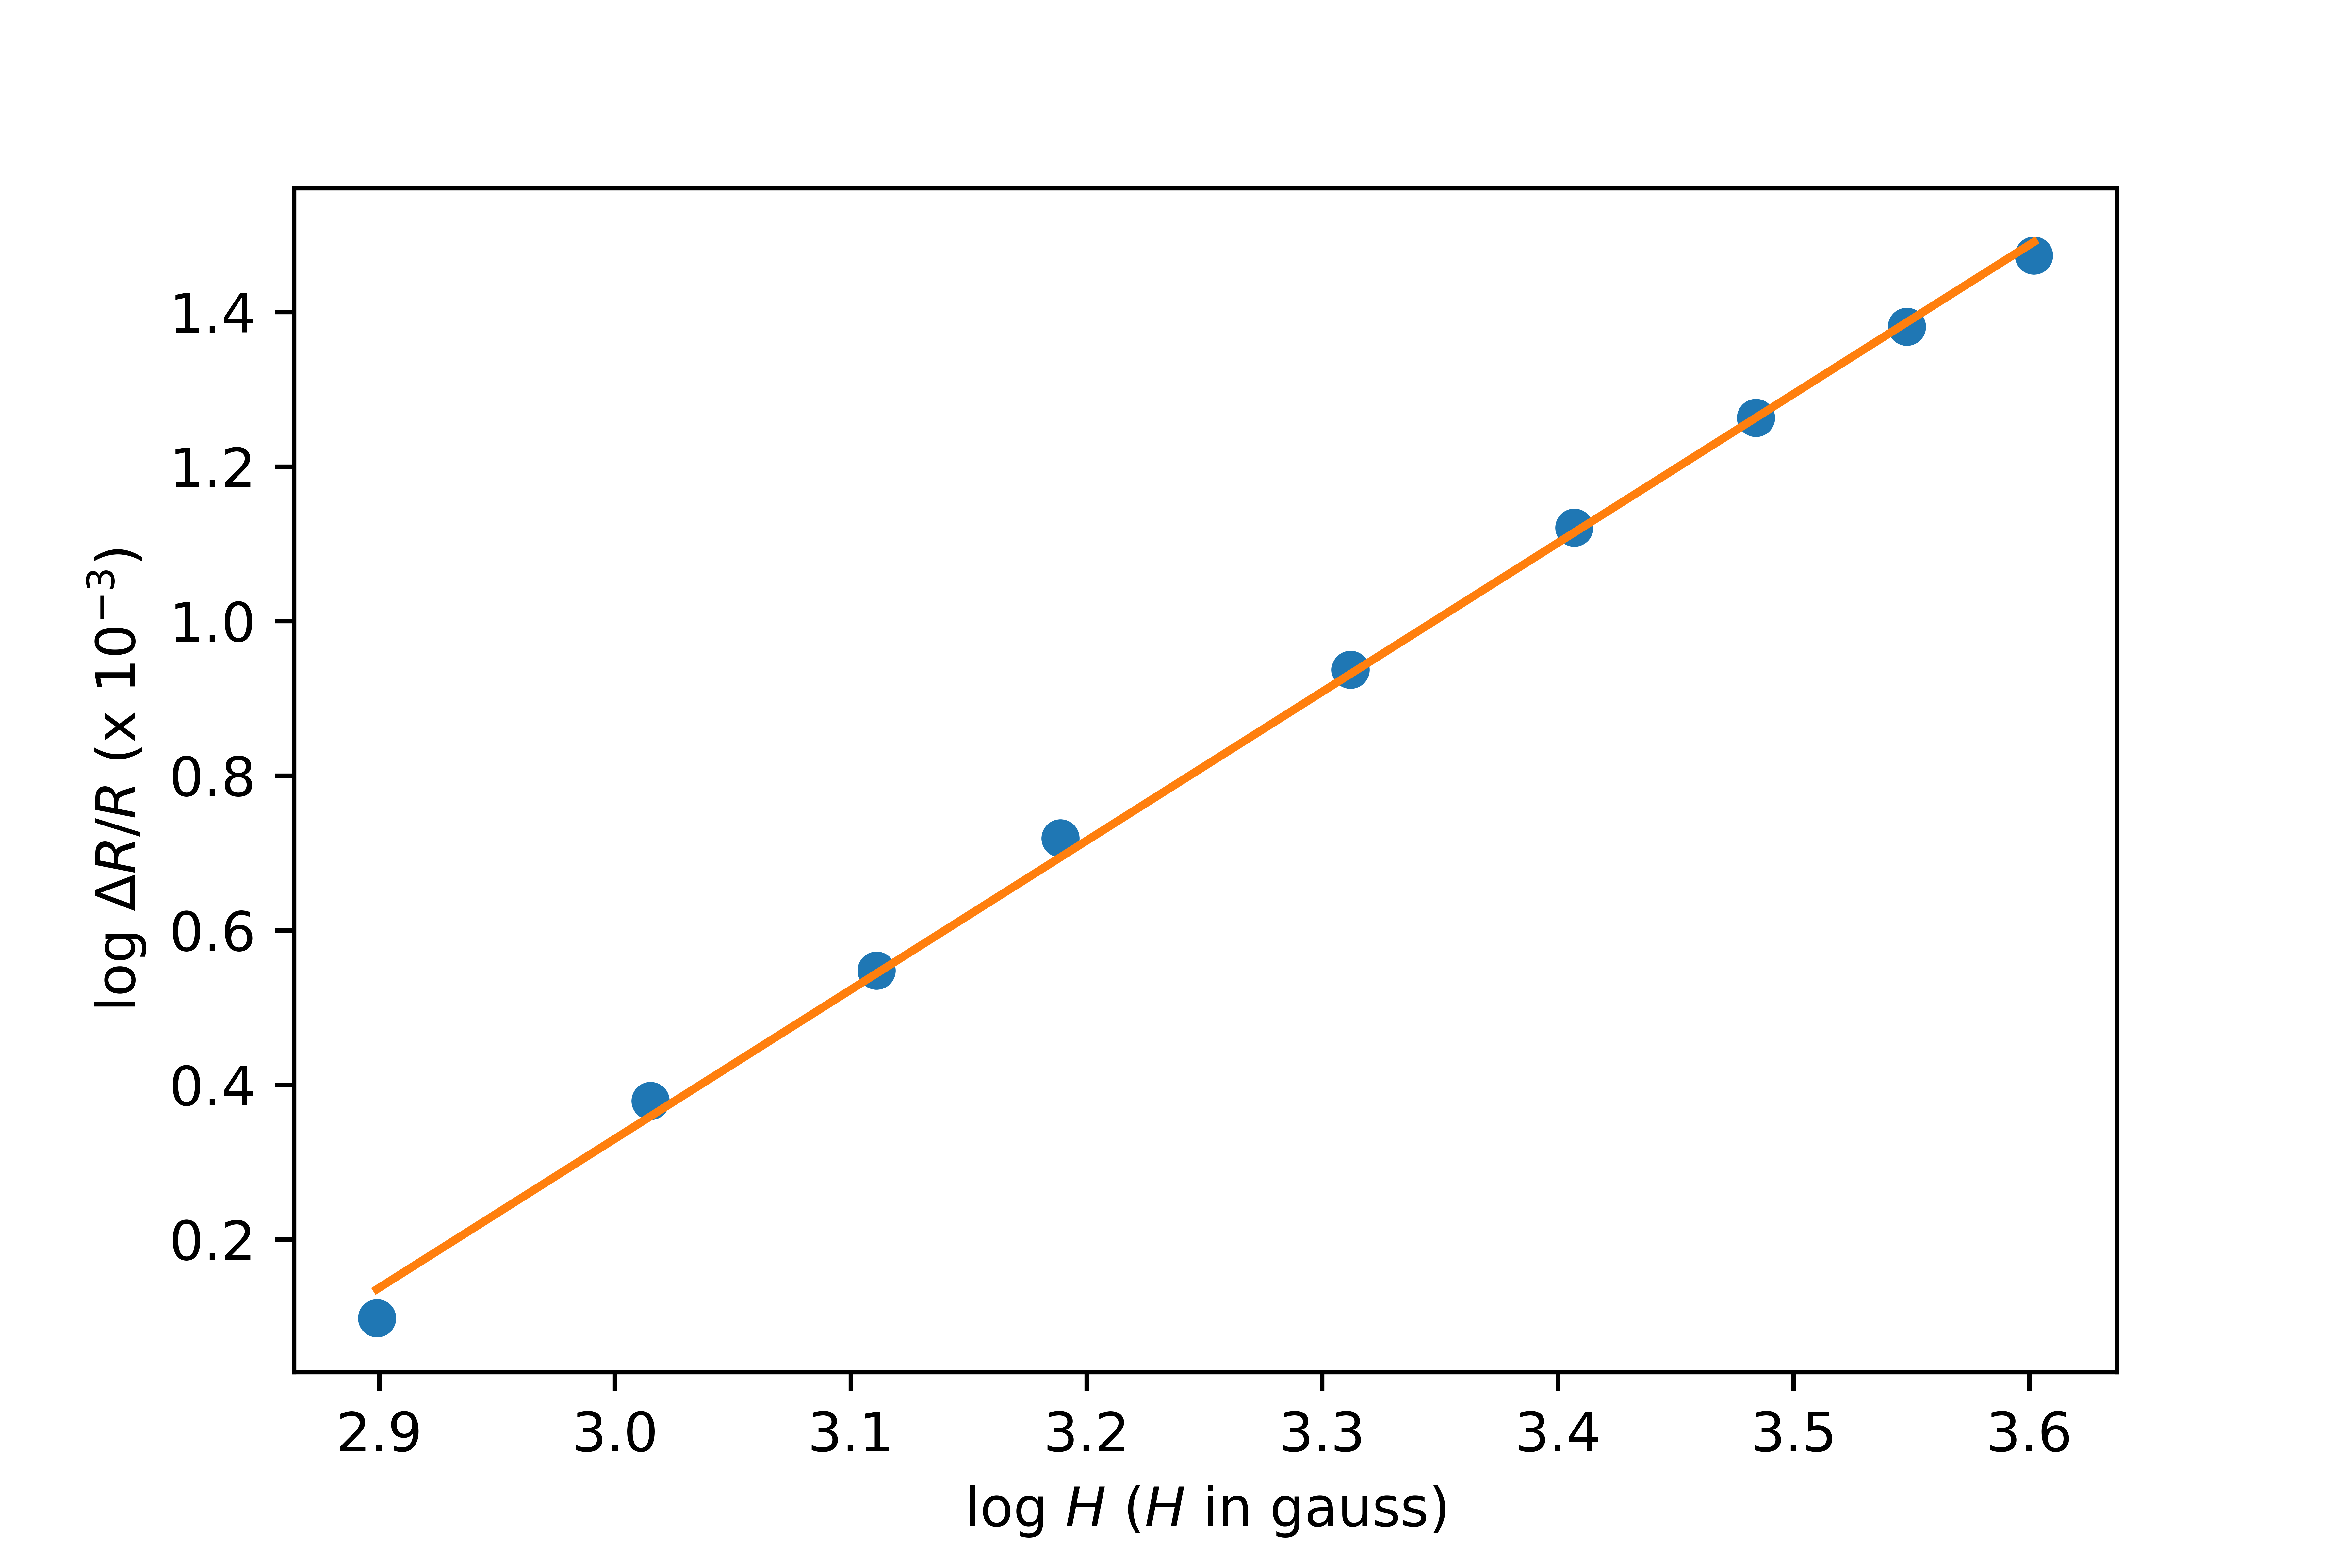
\includegraphics[scale = 0.56]{Figures/plot-mgrst-Ge-log.png}
    \caption{$\log \Delta R/R \sim \log H$ plot for n-Ge}
    \label{fig:lognGe}
\end{figure}
\begin{figure}
    \centering
    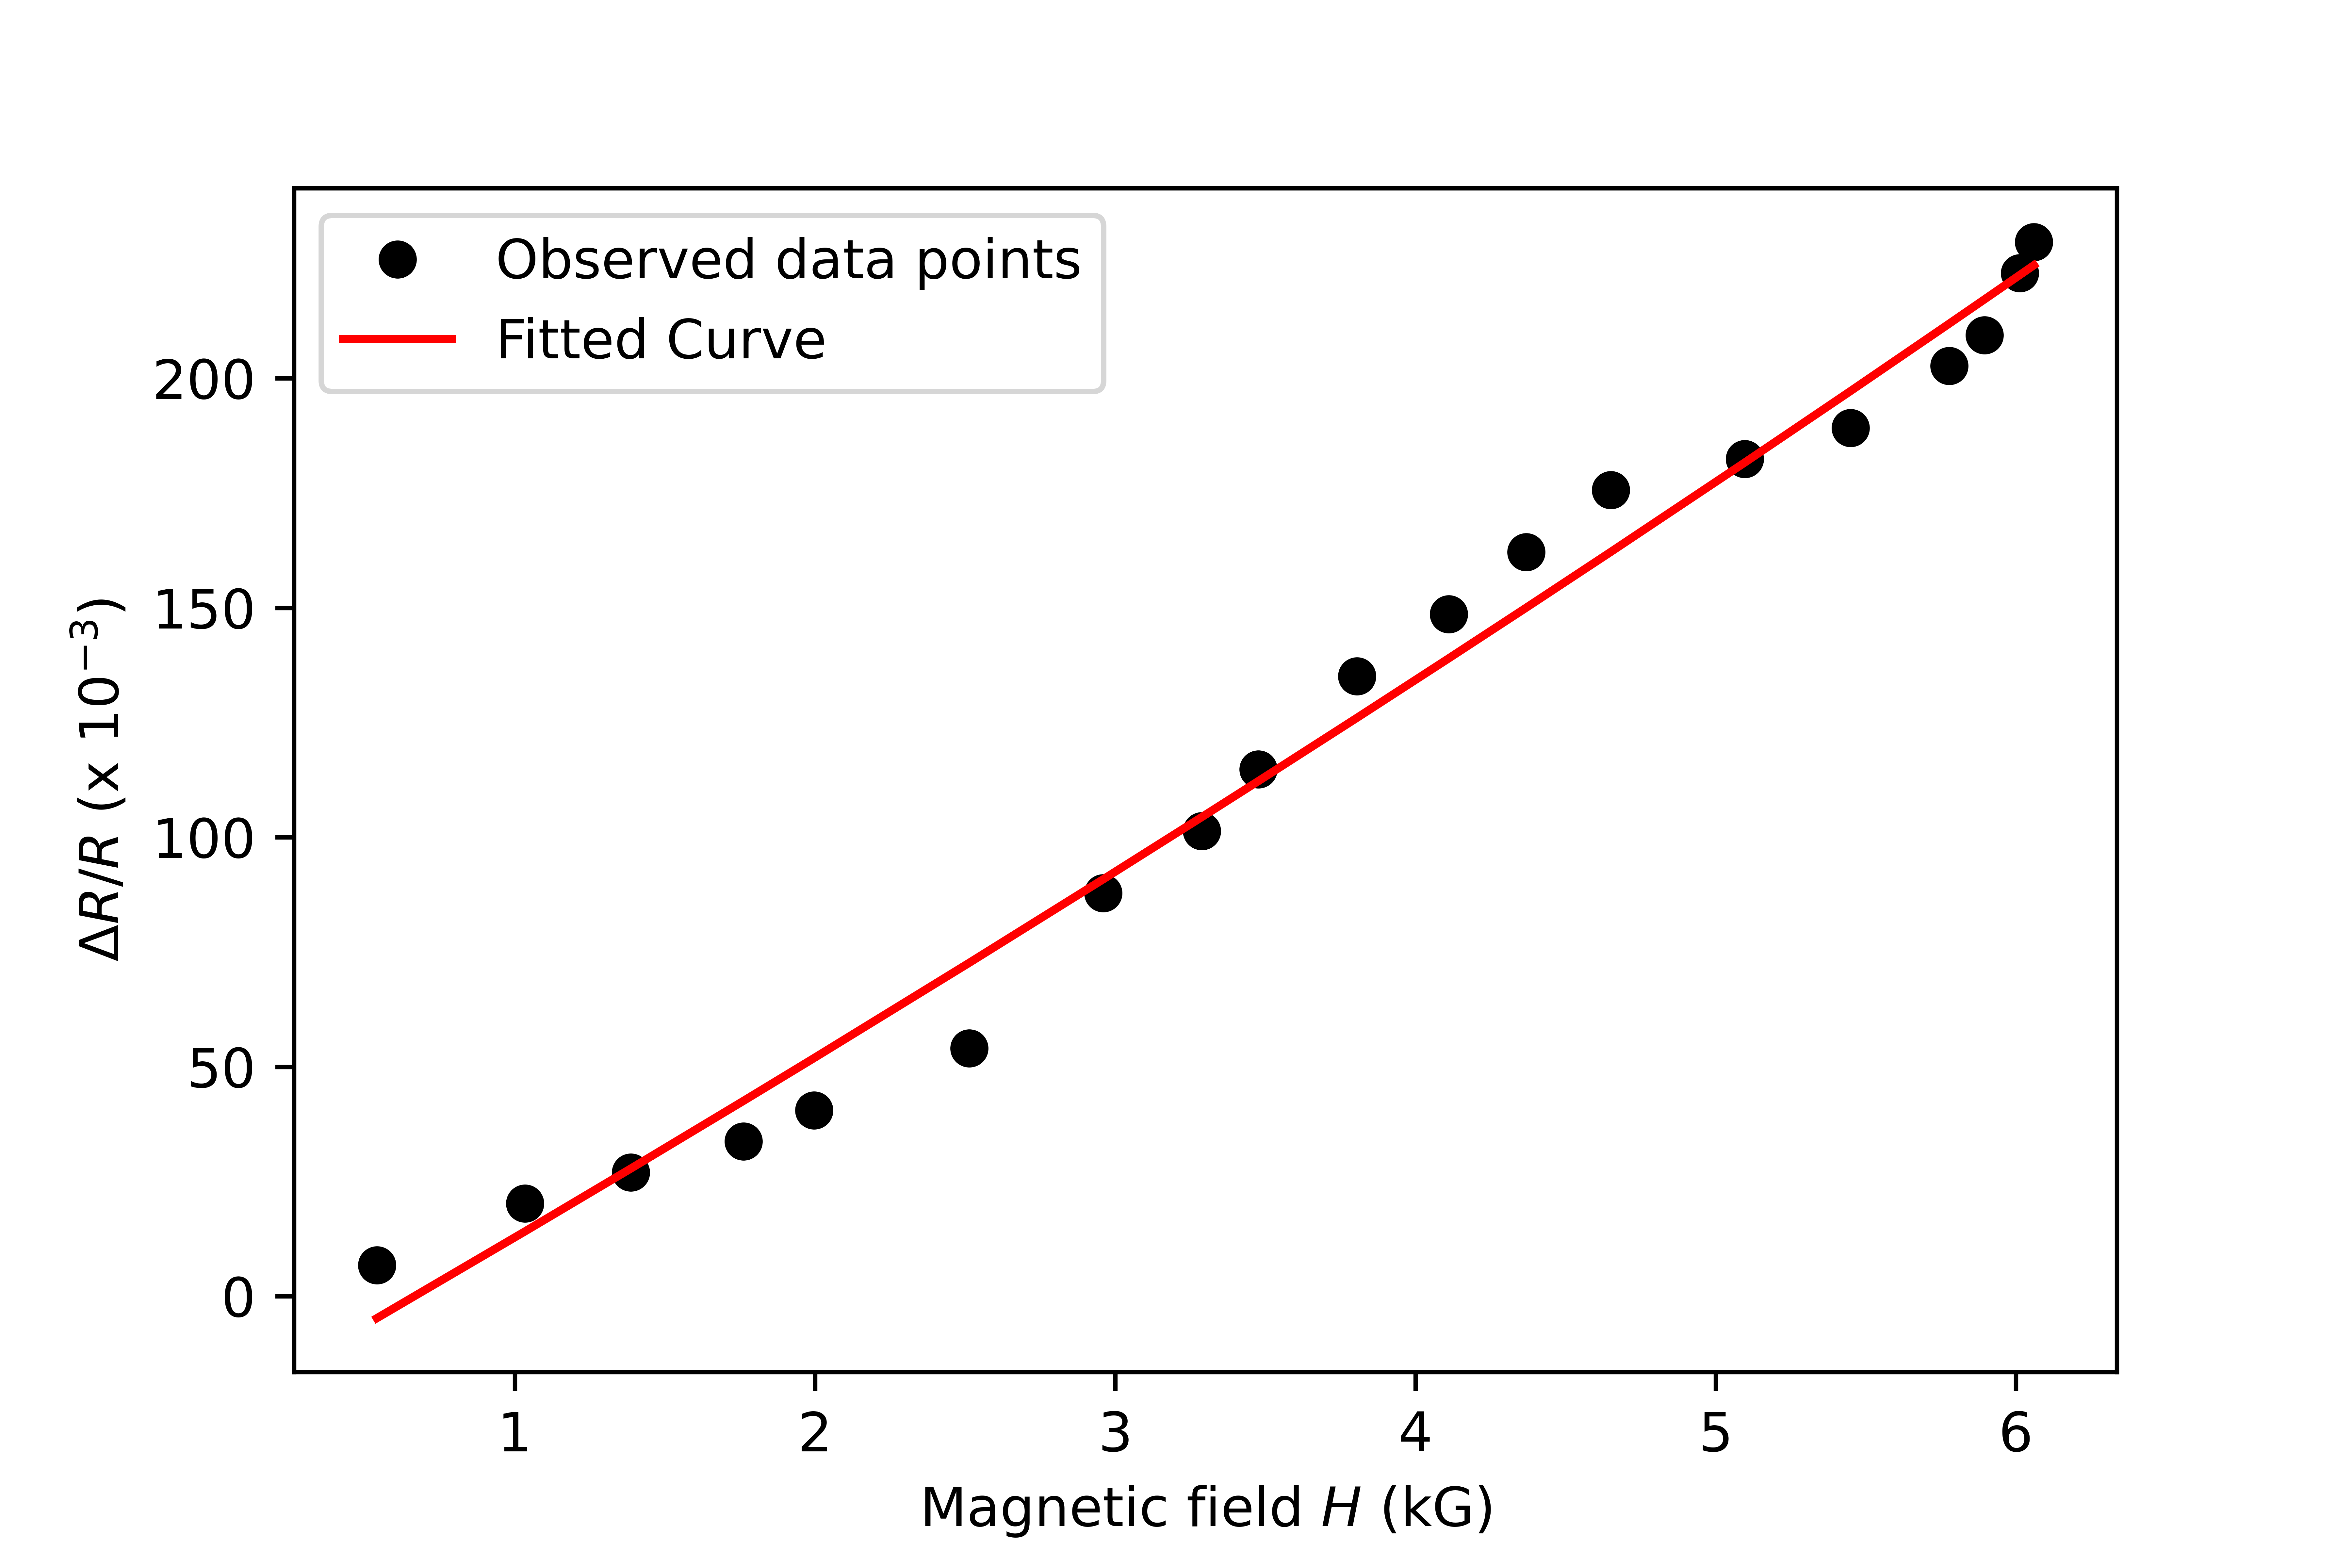
\includegraphics[scale = 0.56]{Figures/plot-mgrst-Bi.png}
    \caption{$\Delta R/R \sim H$ plot for Bi}
    \label{fig:bimgst}
\end{figure}
\begin{figure}
    \centering
    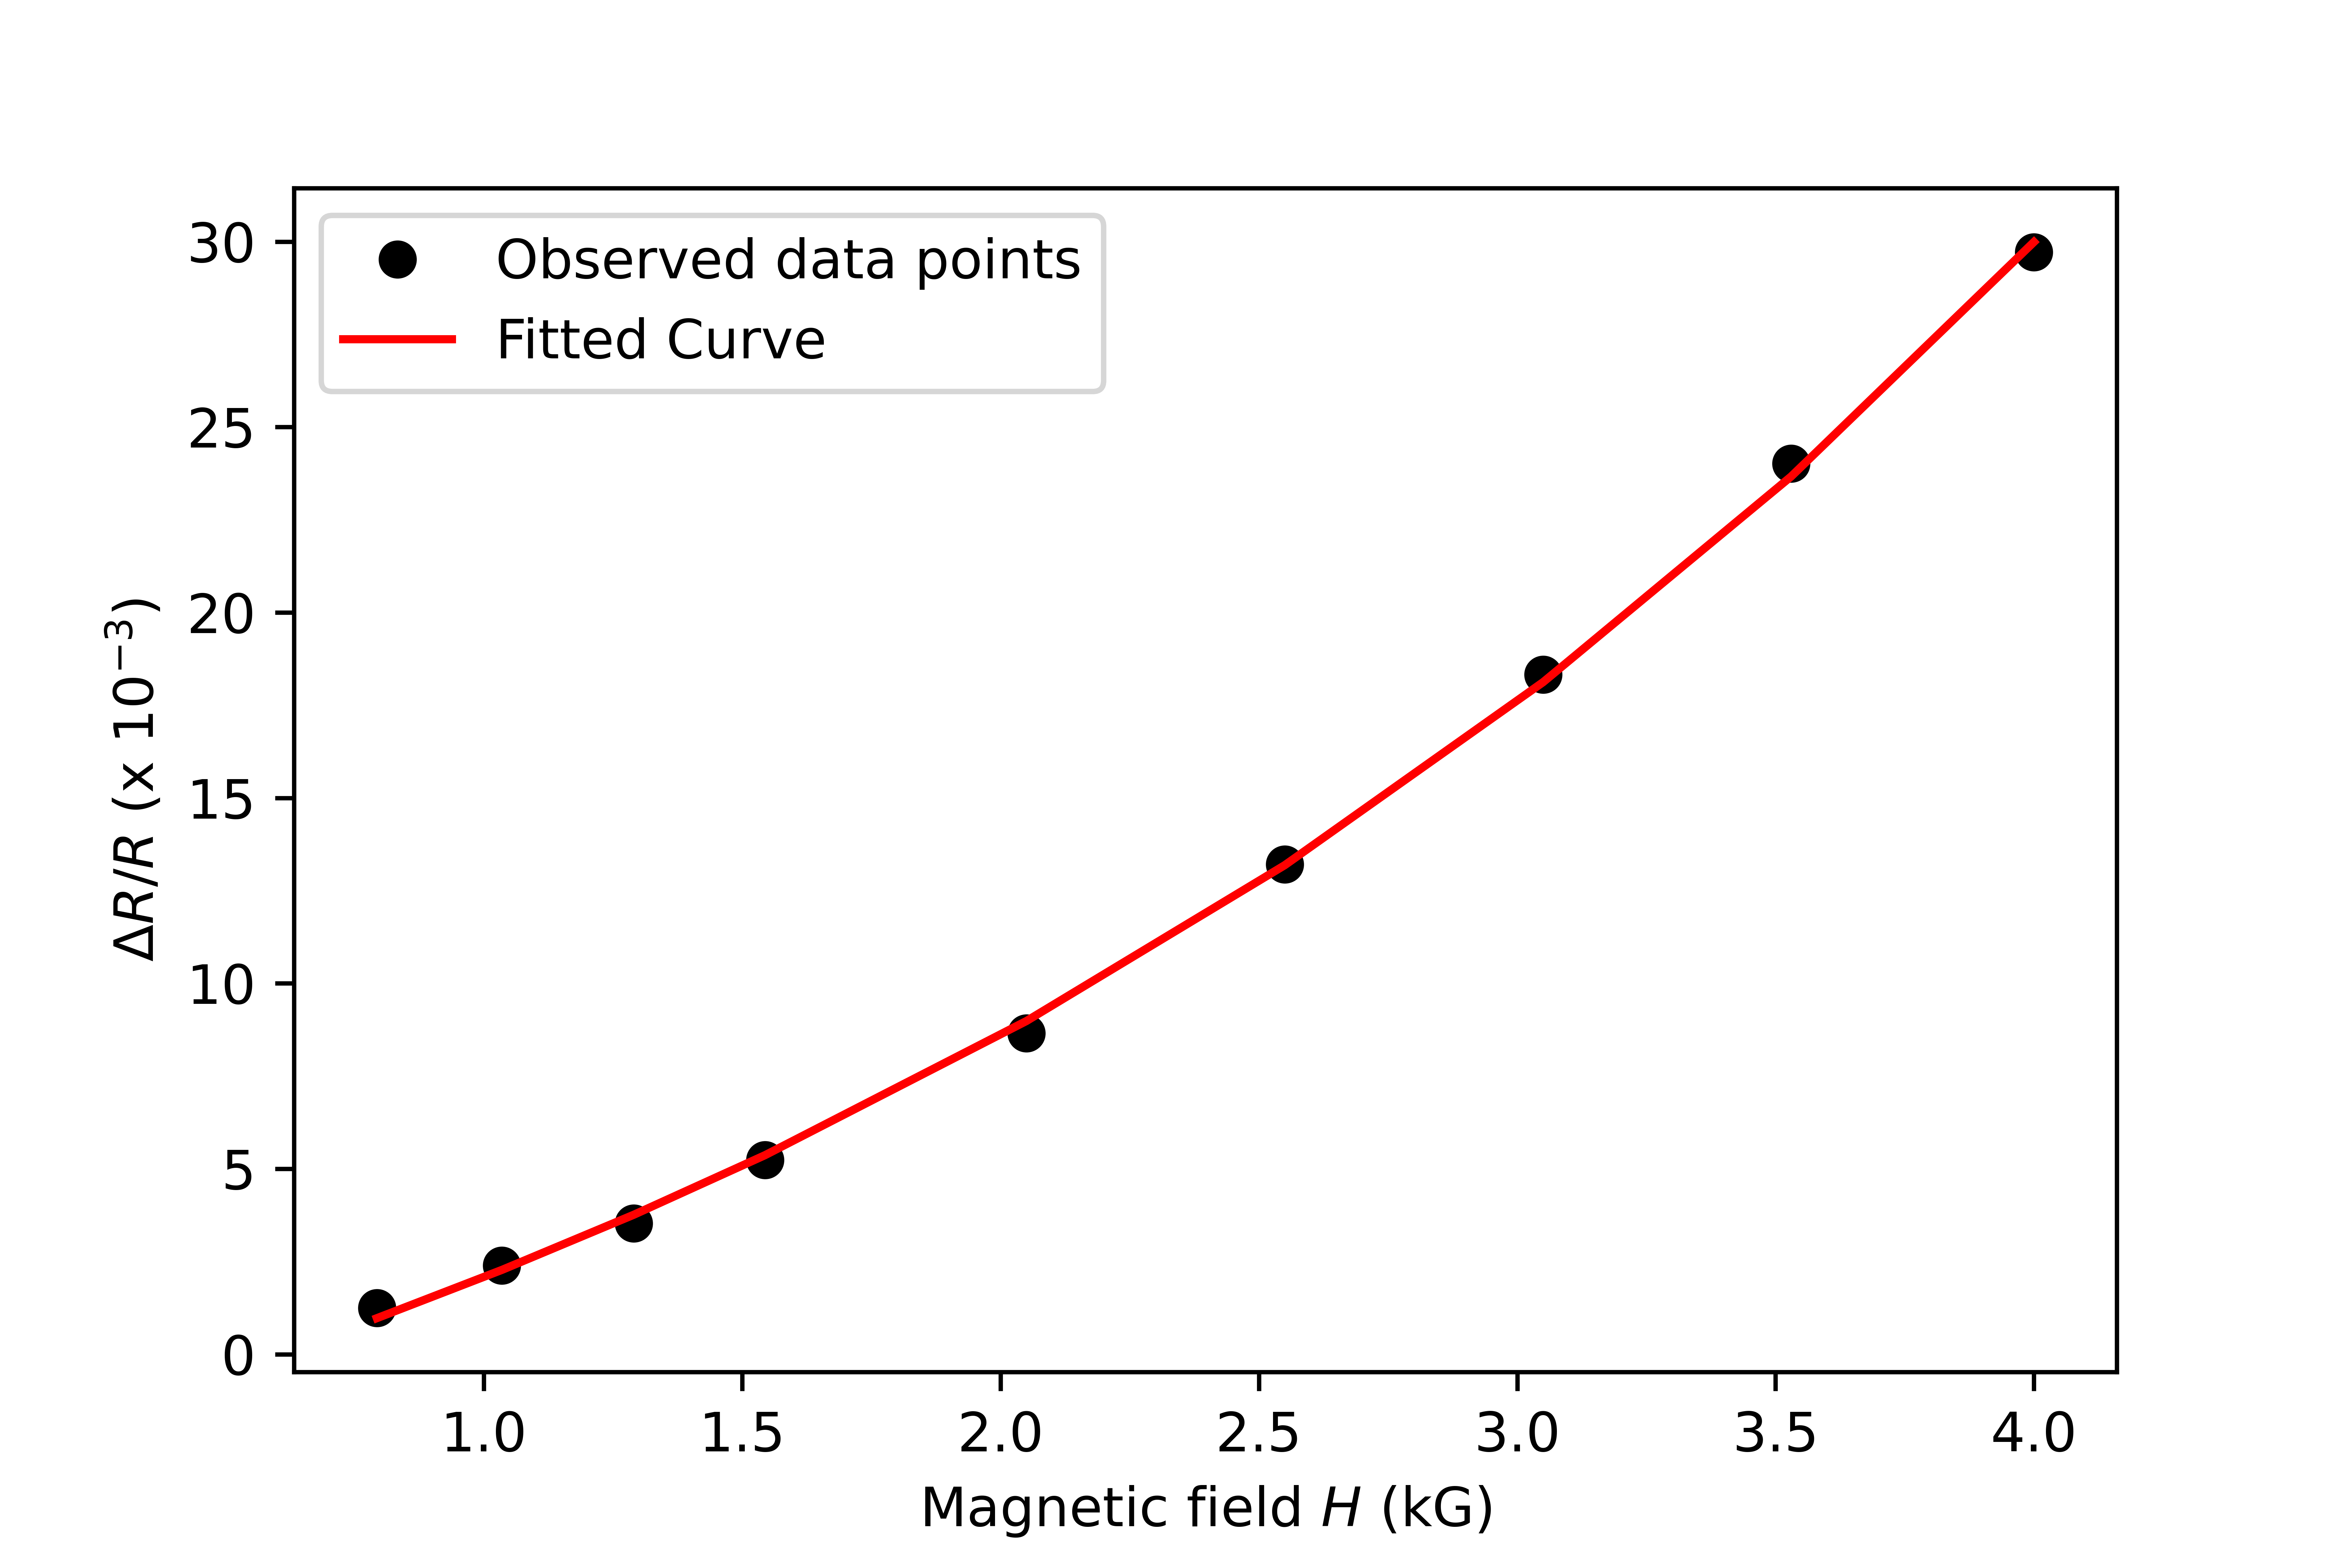
\includegraphics[scale = 0.56]{Figures/plot-mgrst-Ge.png}
    \caption{$\Delta R/R \sim H$ plot for n-Ge}
    \label{fig:nGemgrst}
\end{figure}
\section{Calculations}
We have, Hall coefficient 
\begin{equation}
\label{hallR}
    R = \dfrac{V_h z}{IH}
\end{equation}
The slope of the $V_h \sim H$ for Bi by using the data given in table (\ref{tab:bihall}) is $\SI{4.23e-6}{\milli \volt \per \gauss}$, for p-Ge using data given in table (\ref{tab:hallpGe}) is $\SI{0.0045}{\milli \volt \per \gauss}$ and for n-Ge using the data given in table (\ref{tab:hallnGe}) is $\SI{0.00935}{\milli \volt \per \gauss}$. Putting in the values we get the Hall coefficients as $R_{Bi} = \SI{11.13e-10}{\ohm \centi \metre \per \gauss}$, $R_{p-Ge} = \SI{2.29e-7}{\ohm \centi \metre \per \gauss}$ and $R_{n-Ge} = \SI{3.90e-7}{\ohm \centi \metre \per \gauss}$.
\par
Now the carrier density for Bi is given by
\begin{equation}
    n = \dfrac{1}{R q}
\end{equation}
where $q = \SI{1.6e-19}{\coulomb}$. This gives $n = \SI{5.61e21}{\per \centi \metre \cubed}$.
The carrier mobility is given by
\begin{equation}
    \mu = \dfrac{R}{\rho}
\end{equation}
Putting the values gives us carrier mobility for Bi as $\mu = \SI{8.63e-6}{\centi \metre \squared \per \volt \per \second}$.


\section{Error Analysis}
The error in Hall coefficient is given by
\begin{equation}
    d R = \sqrt{\Big(\dfrac{\partial R}{\partial m} \sigma_{m}\Big)^2 + \Big(\dfrac{\partial R}{\partial z} \sigma_{z}\Big)^2 + \Big(\dfrac{\partial R}{\partial I} \sigma_{I}\Big)^2}
\end{equation}
where $m$ is the slope of the $V_h \sim H$ curve for the semiconductor.
Now error in slope, $\sigma_m$ is given by
\begin{equation}
    \sigma_m = \sigma_y \sqrt{\dfrac{n}{\Delta}}
\end{equation}
Here $\sigma_y$ is the least count of $V$ and $n$ and $\Delta$ represent the usual summations in regression analysis.
After putting the values and solving, we get error in Hall voltage for Bi $d R_{Bi} = \SI{0.03e-10}{\ohm \centi \metre \per \gauss}$. Similarly we get $d R_{p-Ge} = \SI{0.03e-7}{\ohm \centi \metre \per \gauss}$ and $d R_{n-Ge} = \SI{0.02e-7}{\ohm \centi \metre \per \gauss}$.
\par
Error in carrier density $n$ is only due to $R$, and is equal to $dn = \SI{0.17e21}{\per \centi \metre \cubed}$ and similarly, error in carrier mobility is also just due to $R$ and is equal to $d \mu = \SI{0.27e-6}{\centi \metre \squared \per \volt \per \second}$.



\section{Results}
\begin{enumerate}
    \item The Hall coefficient of Bi is given by $\SI[separate-uncertainty=true]{11.13 \pm 0.03e-11}{\ohm \centi \metre \per \gauss}$.
    \item The Hall coefficient of p-Ge is given by $\SI[separate-uncertainty=true]{2.29 \pm 0.03e-7}{\ohm \centi \metre \per \gauss}$.
    \item The Hall coefficient of n-Ge is given by $\SI[separate-uncertainty=true]{3.90 \pm 0.02e-7}{\ohm \centi \metre \per \gauss}$.
    \item The carrier density for Bi is $n = \SI[separate-uncertainty=true]{5.61 \pm 0.17e21}{\per \centi \metre \cubed}$.
    \item The carrier mobility for Bi  is $\mu = \SI[separate-uncertainty=true]{8.63 \pm 0.27e-6}{\centi \metre \squared \per \volt \per \second}$.
    \item The log-log graphs between magnetic field and $\Delta R/R$ were straight lines and graphs between $\Delta R/R$ and $H$ were exponential.
\end{enumerate}

\section{Discussions}
\begin{enumerate}
    \item The hall coefficient for Bismuth and n-Ge comes out as negative as was expected. This signifies the majority charge carriers are electrons.
    \item The hall coefficient for p-Ge is positive as was expected. This signifies that holes are the majority charge carriers.
    \item The resistance of the sample increases with the increase in the magnetic field as evident by the formula.
    \item A high voltage impedance is generally needed to measure the Hall voltage.
    \item The Hall voltage should be measured for both directions of current as well as magnetic field.
    \item With increase in temperature, the Hall voltage falls in value and turns negative soon after.
    \item Magneto-resistance is explained qualitatively using cyclotron effect in metals which devoid of magnetic moment and with spin disorder in magnetic atoms. Bismuth comes under first category.
    \item The plots for magneto-resistance were obtained as expected, although the plot for Bi had an inflection point, which implies poor data.
    \item The logarithmic graph follows a straight line as expected.
\end{enumerate}

\section{Conclusions}
\begin{enumerate}
    \item In most cases, the results so obtained were satisfactory.
    \item As the resistivity of the sample of n-Ge and p-Ge was not known, carrier mobility could not be calculated for them.
    \item Error could have been obtained due to carrier injection or improper doping of the sample.
\end{enumerate}

\nocite{*}
%\bibliography{bibliography}% Produces the bibliography via BibTeX.

\end{document}
%
% ****** End of file aipsamp.tex ******